% !TEX encoding = IsoLatin2
%spellcheck-off
\documentclass[Bachelor, BIC, german]{twbook}

\usepackage[T1]{fontenc}
% Hier kann je nach Betriebssystem eine der folgenden Optionen notwendig sein, 
% um die Umlaute korrekt wiederzugeben: utf8, latin, applemac
\usepackage[utf8]{inputenc}

% Einstellungen für Zitate
\usepackage{csquotes}

\DeclareQuoteStyle[quotes]{german}
  {\itshape\textquotedblleft}
  [\textquotedblleft]
  {\textquotedblright}
  [0.05em]
  {\textquoteleft}
  {\textquoteright}

% Hack zum stillegen der hyperref babel redefine warnings
\makeatletter
\patchcmd{\pdfstringdef}
  {\csname HyPsd@babel@}
  {\let\bbl@info\@gobble\csname HyPsd@babel@}
  {}{}
%\makeatother

\usepackage[activate={true,nocompatibility},final,tracking=true,kerning=true,spacing=true,factor=1100,stretch=10,shrink=10,babel]{microtype}

\usepackage{wrapfig}
\usepackage{enumitem}

% Bibliografie Einstellungen
\usepackage{biblatex}
\bibliography{literatur}
\renewcommand*{\bibfont}{\footnotesize}

%Formatieren des Quellcodeverzeichnisses
\usepackage[final]{listings}
\usepackage{color}

\definecolor{mygreen}{rgb}{0,0.6,0}
\definecolor{mygray}{rgb}{0.5,0.5,0.5}
\definecolor{mymauve}{rgb}{0.58,0,0.82}

\lstset{captionpos=b, numberbychapter=false,caption=\lstname,frame=single, numbers=left, numberstyle=\tiny\color{mygray}, stepnumber=1, numbersep=5pt, xleftmargin=10pt, numberstyle=\tiny, tabsize=2, columns=fixed, basicstyle={\fontfamily{pcr}\selectfont\footnotesize}, keywordstyle=\bfseries, commentstyle=\color{mygreen}, keepspaces, breaklines, breakatwhitespace, breakautoindent
}

%\makeatletter
% Setzen der Bezeichnungen für das Quellcodeverzeichnis/Abkürzungsverzeichnis in Abhängigkeit von der eingestellten Sprache
\providecommand\listacroname{}
\renewcommand\lstlistingname{Quellcode}
\renewcommand\lstlistlistingname{Quellcodeverzeichnis}
\renewcommand\listacroname{Abkürzungsverzeichnis}

% Einstellungen der Class TWBOOK
\title{DNS Client Security\\Bedrohungen und Lösungswege}
\author{Michael Riedmann}
\studentnumber{1510258054}
\supervisor{FH-Prof. Dipl.-Ing. Alexander Mense}
\place{Wien}

\kurzfassung{% Wird vom Template eingefügt, kein Chapter oder so einfügen!

Das Ziel dieser Arbeit war es, Lösungsmöglichkeiten für aktuelle Sicherheitsprobleme der Domain Name Systems (DNS) näher zu untersuchen. DNS, als zentrales Namensauflösungs- und Informationssystem, stellt eine zentrale Komponente des modernen Internets dar. Die Sicherheit des Internets ist daher eng an die des DNS gebunden. Mit Hilfe der bestehenden Literatur konnte eine umfangreiche Analyse der relevanten Bedrohungen und deren Mitigarionsmöglichkeiten durchgeführt werden. Basierend auf dieser wurde ein Lösungskonzept ausgearbeitet und über einen Testaufbau validiert. Die durchgeführten Funktions-Tests ergaben, dass der dargestellte Aufbau in der Lage ist, DNS Clients vor allen behandelten Bedrohungen zu schützen. Die Performance-Messungen ergaben eine Verschlechterung der durchschnittlichen Paketumlaufzeit von 5 bis 9\%. Diese Ergebnisse lassen darauf deuten, dass der vorgestellte Aufbau dazu in der Lage ist die Sicherheit maßgeblich zu verbessern, ohne eine starke Verschlechterung der User-Experience zu erzeugen.}
\schlagworte{DNS, DNS Sicherheit, IT-Sicherheit, DNSSEC, DNS-over-TLS}

\outline{%% spellcheck-language "en"

% Wird vom Template eingefügt, kein Chapter oder so einfügen!

The goal of this thesis was the exploration of feasible solutions for current security-issues concerning the Domain Name System (DNS). As internet security is tightly connected with DNS security, this is an important topic to investigate. A thorough research of current literature was conducted to determine relevant threats and possible mitigation strategies. Based on this analysis, a proof-of-concept was developed. The evaluation showed that the proposed setup is able to protect DNS Clients from all threads disscused in this thesis. Performance tests reported an increase in the average round-trip-time by only 5-9\%. These results indicate that implementing the proposed approach substantially improves security without significantly decreasing the overall user-experience.}
\keywords{DNS, DNS Security, IT-Security, DNSSEC, DNS-over-TLS}

% Allgemeine Einstellungen
\pretolerance=1500
\tolerance=2000 
\emergencystretch=10pt

\setkomafont{caption}{\footnotesize\itshape}
\setkomafont{captionlabel}{\usekomafont{caption}}

\graphicspath{ {./PICs/} }
\DeclareGraphicsExtensions{.pdf,.png}
\setlength{\belowcaptionskip}{-0.5\baselineskip}

% --------------------------------------------------------------------------- %
\begin{document}
\maketitle

\RedeclareSectionCommand[
  beforeskip=-1pt plus -16pt minus -1pt,
  afterskip=.5\baselineskip]{chapter}
\RedeclareSectionCommand[
  beforeskip=-1em plus -3em minus -1pt,
  afterskip=.25\baselineskip]{section}
\RedeclareSectionCommand[
  beforeskip=-.25\baselineskip,
  afterskip=.1\baselineskip]{subsection}
%\RedeclareSectionCommand[
%  beforeskip=-.25\baselineskip,
%  afterskip=1pt]{subsubsection}
%\RedeclareSectionCommands[
%    beforeskip=-1.2ex plus -1ex minus -0.2ex,
%    afterskip=1sp,% smallest possible positive value
%]{paragraph,subparagraph}

\chapter{Einleitung}
Das \ac{DNS} bietet eine einfache Möglichkeit zur Namesauflösung und damit die Grundlage für menschenles- und merkbare Namen in modernen Computernetzwerken. Außerdem dient es als verteilte Datenbank für simple Informationen über Netzwerke und Hosts. Speziell im Internet nimmt dieses Service somit eine zentrale Rolle im Verbindungsaufbau zwischen den vernetzen Systemen ein. Betrachtet man das Netzwerkprotokoll des DNS genauer, stellt man fest, dass es ohne jegliche Ansprüche an Informationssicherheit konzipiert wurde. Dieser Umstand ist seinem Alter geschuldet, widerspricht damit aber dennoch den heutigen IT-Sicherheitsstandards. Zur Erfüllung dieser Ansprüche wurden in den letzten Jahrzehnten verschiedene Ansätze zur Verbesserung dieser Situation entwickelt. Trotzdem hat es bis zum heutigen Tag keiner der entwickelten Standards geschafft, eine weitreichende Durchdringung zu erlangen. Obwohl das Bedürfnis nach Sicherheit über die Zeit stark gestiegen ist, trägt speziell DNS in seinem momentanen Zustand mehr zur Verschärfung der Lage als zu dessen Entschärfung bei.

Diese Arbeit beschäftigt sich mit der Analyse der aktuellen Situation und präsentiert einen möglichen Lösungsvorschlag. In Kapitel \ref{chap:itsecurity} werden zur Einführung in das Thema Informations- und IT-Sicherheit die wichtigsten Begrifflichkeiten vorgestellt. Trotzdem wird in diesem und folgenden Kapiteln von einem grundlegenden Verständnis der Bereiche Systemtechnik, Netzwerktechnik, IT-Sicherheit und Kryptografie ausgegangen. Der Inhalt dieser Arbeit ist daher an erfahrene SystemadministratorInnen, ohne spezielle Erfahrung im Bereich DNS-Sicherheit gerichtet. Um das notwendige Vorwissen im Bereich DNS zu vermitteln, wird in Kapitel \ref{chap:dns} eine kurze Einführung in die Funktionsweise von DNS gegeben. Darüber hinaus werden die sicherheitsrelevanten Aspekte des Systems (siehe Abschnitt \ref{sec:dnssecurity}) näher erläutert. 

Den Kern der Arbeit stellt eine detaillierte Darstellung der aktuellen Sicherheitsprobleme und mögliche Lösungen, mit Fokus auf Endgeräte und User, dar. Dazu werden, in Kapitel \ref{chap:threads}, die wichtigsten Bedrohungen behandelt. Um diese besser zu verstehen, sind in Kapitel \ref{chap:attacks} die häufigsten Angriffsmethoden beschrieben. Basierend auf diesen werden logisch gefolgerte, sowie in anderen Arbeiten vorgeschlagene, allgemeine Lösungsvorschläge abgegeben (Kapitel \ref{chap:solutions}). 

Um diesen Empfehlungen einem praktischen Nutzen zuzuführen werden in Kapitel \ref{chap:technologies} aktuell verfügbaren Technologien vorgestellt, die zur Umsetzung dieser Konzepte herangezogen werden können. Die Gesamtheit der erarbeiteten Informationen fließt in einem, unter Kapitel \ref{chap:implementation} beschriebenen, Test-Aufbau zusammen. Dieser stellt eine Möglichkeit zur Erfüllung der formulierten Ziele unter Zuhilfenahme bestehenden Technologien dar. Die Resultate mit speziellem Fokus auf Performance werden in Kapitel \ref{chap:results} vorgestellt und in einem abschließenden Fazit diskutiert.


\chapter{Sicherheit in der IT}
\label{chap:itsecurity}
Da sich diese Arbeit größtenteils mit Sicherheit beschäftigt, ist es notwendig dieses Thema bewusst einzugrenzen und mögliche Mehrdeutigkeiten vorab zu klären.

\section{Allgemeine Definitionen}
Um ein einheitliches Verständnis zu erzielen, werden in diesem Kapitel die wichtigsten Begriffe kurz definiert.

\paragraph{Informationssicherheit}
Wie das \ac{BSI} in seinem Glossar darlegt, hat Informationssicherheit den Schutz von Informationen als Ziel\cite{BSIGlossar}. Dieser Begriff ist bewusst nicht auf digitale Daten oder Computer beschränkt, sondern umfasst alle Arten von Informationen. Um Informationssicherheit zu erreichen werden drei Schutzziele definiert: Vertraulichkeit (engl. confidentiality), Integrität (engl. integrity) und Verfügbarkeit (engl. availability).

\paragraph{Vertraulichkeit}
Informationsvertraulichkeit von Daten und Systemen ist gegeben, wenn keine unautorisierte Informationsgewinnung möglich ist\cite[p. 10]{Eckert2013}. Dieser Definition spart bewusst die Möglichkeit auf Veränderung oder den Besitz aus. Es ist also durchaus möglich, blinde Änderungen an Daten zuzulassen oder eine unautorisierte Partei in Besitz der Daten kommen zu lassen, solange es nicht möglich ist die darin enthaltenen Informationen zu extrahieren. Dieses Szenario ist in den meisten verschlüsselten Netzwerkübertragungen durchaus der Fall und verletzt den Begriff der Vertraulichkeit noch nicht.    

\paragraph{Integrität}
Datenintegrität ist gewährleistet, wenn eine unautorisierte und unbemerkte Veränderung von Daten unmöglich ist\cite[p. 9]{Eckert2013}. Dabei liegt der Schwerpunkt, speziell im Bereich der Netzwerktechnik, auf dem Erkennen von Veränderung, statt deren Verhinderung. Wird eine Veränderung zuverlässig erkannt, ist Integrität bereits gegeben. Das Gewährleisten der Integrität garantiert dabei keine Vertraulichkeit und umgekehrt.

\paragraph{Verfügbarkeit}
Verfügbarkeit behandelt die Nutzbarkeit eines Systems durch berechtigte Subjekte. Dabei darf es nicht zu einer unautorisierten Verweigerung des Zugriffs kommen \cite[p. 12]{Eckert2013}. Dies beinhaltet z.B. auch einen hardwarebedingten Ausfall eines Systems, schließt aber bewusst den aktiven Eingriff von Außen nicht aus.
 
\paragraph{Authentizität}
Ein abgeleitetes Schutzziel stellt dabei die Authentizität (engl. authenticity) dar. Diese ist gegeben, wenn ``die Echtheit und Glaubwürdigkeit des Objekts bzw. Subjekts, [...] anhand einer eindeutigen Identität und charakteristischen Eigenschaften überprüfbar ist''\cite[p. 8]{Eckert2013}. Der Vorgang der Feststellung der Authentizität wird Authentifizierung genannt. Dabei wird die behauptete Identität unter Zuhilfenahme einer charakteristischen Eigenschaft verifiziert. Ein einfaches Beispiel ist dabei die Eingabe eines Passwortes, bei dem die behauptete Identität, also die Benutzerkennung, über die charakteristische Eigenschaft, das Wissen es Passwortes, überprüft wird.  

\paragraph{Datenschutz}
Das Konzept des Datenschutzes (engl. Privacy) wird in verschiedenen Quellen unterschiedlich definiert. Im Zuge dieser Arbeit genügt eine vereinfachte Betrachtungsweise. Dabei ist Datenschutz als Schutz vor dem Missbrauch personenbezogener Daten zu verstehen. Die Festlegung was denn nun personenbezogene Daten seien variiert leicht. Auch hier ist es für diese Arbeit ausreichend festzustellen, dass es sich bei Daten die einen Rückschluss auf die Identität einer Person zulassen um personenbezogene Daten handelt. Dazu gehören explizit Adressen (auch IP-Adressen), sowie jede Form von einfach verknüpfbarer ``Online-Kennung''\cite{Schwenke2018}.     

\paragraph{Verbindlichkeit}
Als verbindlich, auch zuordenbar (Zuordenbarkeit; engl. accountability) bzw. nicht-abstreitbar (Nicht-Abstreitbarkeit; engl. non-repudiation), werden Aktionen bezeichnet, deren Durchführung vom durchführenden Subjekt im Nachhinein nicht abgestritten werden kann. Diese Eigenschaft bildet die Grundlage verschiedenster Dienstleistungen, da sie dazu in der Lage ist einzelne Personen an ihre Handlungen zu binden. Man denke an Online-Zahlungen oder das Einreichen offizieller Formulare. Obwohl nicht zwingend notwendig, macht Verbindlichkeit oft nur bei hergestellter Authentizität Sinn und kann daher als untergeordnetes Schutzziel verstanden werden.

\section{Vertrauen}
\label{sec:trust}
Vertrauen (engl. Trust) hat verschiedenste Bedeutungen. In dieser Arbeit wird er jedoch in einem sehr spezifischen Kontext, der asymmetrischen Kryptografie, verwendet. Das Vertrauen liegt dabei in der Fähigkeit eines Merkmals, die Identität einer Person auch wirklich zu beweisen. Es baut damit auf der Definitionen von Authentizität und Verbindlichkeit auf\cite{Perrin2010}. Erlaubt man nun die eigennützige Spezifizierung, so beschreibt Vertrauen die Glaubwürdigkeit der Beziehung zwischen einem kryptografischen Schlüssel und der Identität der ihn besitzenden Person. Um diese Vertrautheit herzustellen, existieren nun verschiedene Möglichkeiten. Diese werden hier als ``Prozesse zur Herstellung einer Vertrauensstellung'' (engl. Trust-Establishment-Process) bezeichnet. Nachfolgend werden die zum Verständnis relevanten Arten beschrieben.

\paragraph{Direkt}
Die einfachste Methode um eine Vertrauensstellung zwischen zwei Parteien herzustellen, ist die direkte Methode. Dabei wird jede Partei über bekannte Merkmale von der jeweils andere authentifiziert. Dies passiert zum Beispiel beim persönlichen Überreichen einer Abschrift der jeweiligen Schüssels. Die Authentifizierung kann dabei über visuelle, auditive oder haptische Merkmale erfolgen.

\paragraph{Trust-On-First-Use}
Das \ac{TOFU} Konzept folgt der Annahme, dass ein Angreifer nur ein begrenztes Zeitfenster besitzt. Dadurch ist es unwahrscheinlich, dass genau die aller ersten Kommunikation zwischen zwei Parteien abgefangen und manipulieren kann. Unter dieser Prämisse ist es sicher die Vertrauensstellung während des ersten Austauschs von Nachrichten herzustellen. Diese Methode ist Nutzenden von \ac{SSH} und \acs{HTTPS} mit selbstsignierten Zertifikaten durchaus geläufig. Wie jedoch festgestellt werden konnte, ist dieses Verfahren von der Verantwortlichkeit der Parteien abhängig und damit als leicht Angreifbar zu werten\cite{Wendlandt2008}.

\paragraph{Chain-Of-Trust}
In der \ac{CoT} wird die Idee des indirekten, transitiven Vertrauens eingeführt. Die bekannteste Umsetzung ist als \ac{PKI} bekannt und liefert die Basis für den sicheren Datenaustausch im \ac{WWW}. Die Verknüpfung eines Schlüssels mit der Identität eines Subjekts wird dabei von einer dritten Stelle, der sogenannten \ac{CA} kontrolliert. Diese führt einen Zertifizierungsprozess  anhand bestimmter charakteristischer Merkmale durch. Bei Erfolg werden die zertifizierten Merkmalen, zusammen mit dem Schlüssel des Subjekts in ein Zertifikat geschrieben und von der \ac{CA} signiert. Will nun eine andere Partei die Echtheit eines von dem Subjekt behaupteten Merkmals prüfen, kann sie über eine Kontrolle des Zertifikats sicher sein, dass eine dritte Partei den Zusammenhang überprüft hat. Was nun zur namensgebenden Kette führt, ist die Frage nach der Vertrauensstellung zu dieser dritten Partei, der \ac{CA}. Dafür gibt es nun zwei Möglichkeiten: Entweder es wurde bereits eine direkte Vertrauensstellung zwischen der \ac{CA} und der prüfenden Partei hergestellt oder die \ac{CA} weist selbst ein Zertifikat einer anderen Stelle vor. Besteht bereits eine Vertrauensstellung, sind damit auch die Zertifikate der Stelle vertrauenswürdig. Herrscht noch kein Vertrauen, wird die ``bürgende Stelle'' untersucht; der Vorgang wiederholt sich; es entsteht eine Kette. Eine Beziehung kann in diesem Konzept dann als vertrauenswürdig angesehen werden, wenn ein Punkt in dieser Kette eine direkte Vertrauensstellung zur prüfenden Partei ausweist. Diesen Punkt wird allgemein als Wurzel (engl. Root) bezeichnet\cite[p. 423 ff.]{Eckert2013}.  


\chapter{DNS}
\label{chap:dns}
DNS bietet ein Service zur standardisierten Auflösung von Ressourcennamen innerhalb globaler oder lokaler Computernetzwerke \cite{rfc1035}. Dabei werden menschenlesbare Zeichenketten (Namen) in Adressen übersetzt. Des Weiteren ist es möglich, zusätzliche Informationen über diese Namen vom System abzufragen.

\section{Aufbau des DNS}
DNS ist als globale Datenbank mit Baum-Struktur konzipiert, welche über eine beliebige Anzahl an vernetzten Rechnern verteilt wird. Der Wurzelknoten der Baums wird dabei als Root bezeichnet und von der \ac{IANA} betrieben. Die Daten dieses Root-Knotens werden über 13 global verteilte Server bereitgestellt. 

Knoten der darunterliegenden und damit ersten Ebene werden als \acp{TLD} bezeichnet und sind nach Ländern (Country-Code TLD; ccTLD) oder Verwendung (Generic TLD; gTLD) gruppiert. Da manche Funktionen von DNS spezielle Domänen benötigen, existiert eine spezielle Infrastruktur-\ac{TLD} (.arpa) die direkt von der \ac{IANA} verwaltet wird. Die anderen TLDs werden von verschiedenen Institutionen betrieben und stellen die höchste Stufe der DNS-Hierarchie dar. Diese sind für die Weitergabe der Verwaltungsrechte der ihnen nachfolgende Unterdomänen, sogenannte \acp{SLD}, verantwortlich. Will nun eine Person das Recht zur Verwaltung einer \ac{SLD} erhalten, muss dies über einen Antrag bei der verwaltenden Stelle oder eines berechtigten Subkontraktors erfolgen. Ist die gewünschte Domäne, z.B. example.com, noch nicht vergeben, werden die Verwaltungsberechtigungen, gegen eine Gebühr, in den Besitz der Antragstellenden übergehen. Alle untergeordneten Domänen sind damit ebenfalls in deren Verantwortung übergegangen. Dieser Aufbau führt zu einer schichtweisen Delegation der Aufgaben innerhalb des globalen DNS-Namensraums (siehe Abb. \ref{img:dnsnamespace}). 

\begin{figure}[!hb]
    \centering
    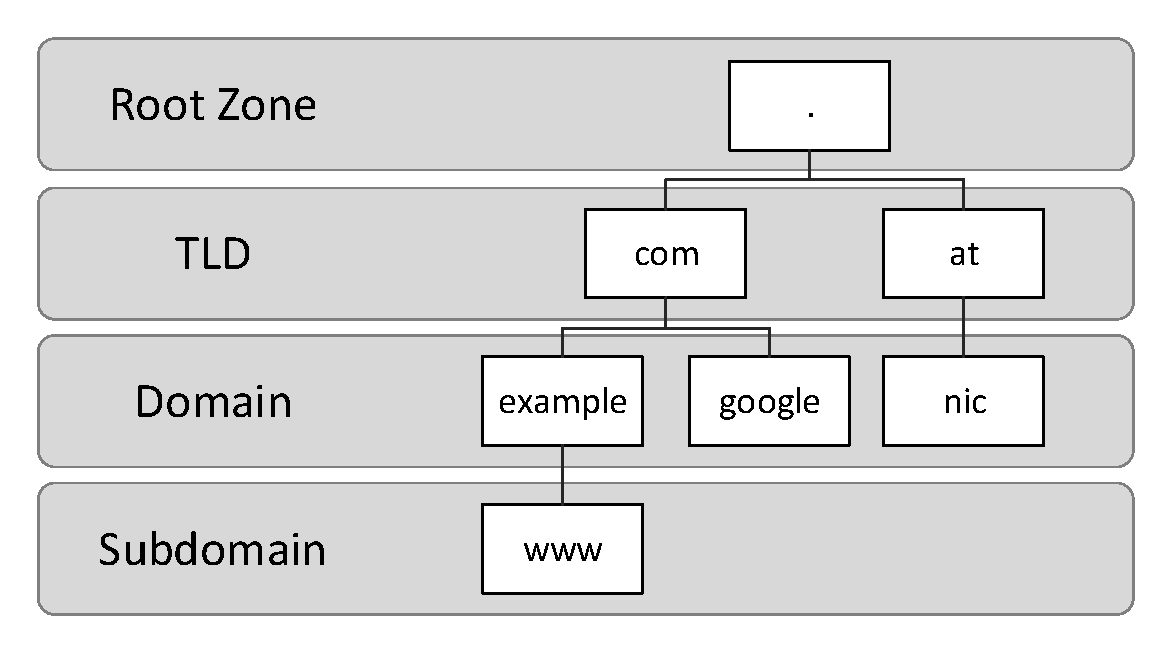
\includegraphics[width=0.5\textwidth]{DNS_NameSpaceLayers}
    \caption{Aufbau des DNS}
    \label{img:dnsnamespace}
\end{figure}

\section{Ressource Records, Sets und Zonen}
Alle Datensätze in DNS werden in einer als \ac{RR} bezeichneter Datenstruktur abgelegt. Ein \ac{RR} besteht dabei aus 5 Informationen: Namen, \ac{TTL}, Klasse (Class), Typ (Type), Datenfeld (Data). Dabei sind die Felder \ac{TTL} und Class optional. Die Menge an Einträgen mit gleichen Werten der Felder Name, TTL, Class und Type bilden dabei ein \ac{RRset}\cite{rfc2181}, das kleinstmögliche abfragbare Element in DNS. Alle \ac{RR} die einem definierten, zusammenhängenden Teil des DNS Namensraum zugeordnet sind, werden als Zone bezeichnet. Diese Sammlung an RR wird in einer Datei, dem \textit{Zone File}, gespeichert und von DNS-Server-Implementationen als Datenbasis genutzt.   

Wie in Listing \ref{lst:dnsZoneFile} zu sehen ist, werden die Daten in einem menschenlesbaren Format gespeichert. Zeile 1 enthält die Anweisung den Namens \texttt{test.example.com.} zu den IPv4-Adressen \texttt{172.30.0.7} und \texttt{172.30.0.8} aufzulösen. Zeile 3 fügt dem Namen weiter Information im Freitextformat hinzu. Zeile 1 und 2 bilden zusammen ein RRset für \texttt{test.example.com 3600 IN A}.

\lstinputlisting[caption={Ausschnitt aus dem Zone-File \textit{example.com}}, label={lst:dnsZoneFile}]{code/example-zone.txt}

\section{DNS Server}
\label{sec:dnsserver}
Um die globale, verteilte Datenbank des DNS nutzen zu können, ist es notwendig, dass diese den DNS-Client-Programmen zugänglich gemacht wird. Das Netzwerkprotokoll ist nach dem klassischen Client-/Server-Konzept ausgestaltet. Es erfordert keinen Verbindungsaufbau und verwendet einen einfachen, sequenziellen Ablauf an Anfragen und Antworten. Ein Client stellt dabei immer nur Anfragen an Server und verarbeitet deren Antwort. DNS-Server können hingegen, je nach Typ, auch selbst Anfragen an andere Server stellen und sind somit nicht nur auf das Beantworten von Anfragen beschränkt. Es können dabei vier unterschiedliche DNS-Server-Typen festgemacht werden.

\paragraph{Stub Resolver}
Die Software, die auf jedem Client-Rechner DNS-Anfragen von Programmen entgegennimmt und diese an die DNS Infrastruktur zur Auflösung übergibt, werden als \textit{Stub Resolver} bezeichnet. Diese können nach außen ausschließlich mit rekursiven Resolvern kommunizieren und nehmen selbst keine DNS-Namensauflösung vor. In manchen Fällen verfügen sie jedoch über einen Cache oder können aufgrund lokaler Policies (z.B. einem Hosts-File) eine Namensauflösung auf anderem Wege durchführen.

\paragraph{Rekursive Resolver}
\textit{Rekursive Resolver} (Recursive Resolver) sind spezielle DNS-Server die von Clients genutzt werden um Namen aufzulösen. Sie verfügen meistens über keine eigenen Zonen und sind damit als Vermittlungskomponente zwischen Endgeräten und den im Internet verfügbaren DNS-Servern zu verstehen.

\paragraph{Autoritative Server}
Server deren Hauptaufgaben im Auflösen von Namen einer oder mehrerer bestimmter Zonen besteht, werden \textit{autoritative Server} (auch Authoritative Server) genannt. Die Bezeichnung spiel auf den Umstand an, dass die Antworten dieses Servers die finale Wahrheit über die von ihm verwalteten Zonen darstellt. Sie lesen die Antworten direkt auf dem Zonen-File der entsprechenden Zone und verlassen sich nicht auf Antworten anderer Server oder Caches. Autoritative DNS-Server stellen damit die Endpunkte der Auflösung für die jeweiligen Domänen dar.

\paragraph{Forwarding DNS Server}
Eine spezielle Form des Rekursive Resolver wird als \textit{Forwarding DNS Server} oder \textit{Forwarding Resolver} bezeichnet. Aus Sicht des Stub Resolvers verhält er sich wie ein gewöhnlicher Rekursiver Resolver. Der Unterschied besteht darin, dass er selbst keinen Auflöse-Prozess durchführt- Die Anfragen werden lediglich an einen anderen Server weiterleitet, welche die eigentliche Auflösung durchführen. Die Ergebnisse werden meist gecacht bevor sie an den Client weitergegeben werden. Dies ist der Grund warum diese Server in seltenen Fällen auch als \textit{DNS-Netzwerk-Cache} oder \textit{Cache-Only Resolver} bezeichnet werden. 

\section{DNS Namensauflösungsprozess}
\label{sec:dnsresolution}
Der Namensauflösungsprozess erfolgt über mehrere Schritte und kann am besten anhand eines Beispiels dargestellt werden. Nehmen wir an, eine Applikation möchte die IPv4-Adresse des Namen \texttt{example.com} herausfinden und stellt eine Anfrage an den lokalen Stub Resolver (kurz Stub) des Client. Der Prozess ist in Abb. \ref{img:dnsresolution} visualisiert und kann Schrittweise wie folgt beschrieben werden:

\begin{enumerate}
    \item Der Stub stellt eine Anfrage nach dem Type A Record der Domäne example.com an den für ihn konfigurierten rekursiven Resolver.
    \item Der Resolver empfängt die Anfrage und prüft seinen lokalen Cache nach dem Eintrag. Da er diesen nicht auffindet wird fortgefahren.
    \item Nun startet der Resolver den rekursiven Auflösungsvorgang. Geht man von einem leeren Cache aus, wird mit der Root-Zone (.) begonnen. Die Anfrage nach www.example.com wird dafür an einen der 13 vorkonfigurierten Root-DNS-Server gesendet.
    \item Der Root-Server empfängt die Anfrage, kann jedoch nur den TLD Teil der Antwort auflösen. Es sendet daher die Adressen des autoritativen Nameserver für die TLD .com zurück.
    \item Der Resolver verarbeitet nun die Adressen und sendet die Anfrage an einen der autoritativen Server der .com Domäne.
    \item Der TLD Nameserver empfängt die Anfrage und prüft, ob für die Domäne example.com eine entsprechende Delegation existiert. Da diese in Form mehrerer NS Einträge vorliegt, wird eine Liste an autoritativen Nameserver-Adressen der SLD Domäne example.com als Antwort gesendet.
    \item Da nun die Adresse eines autoritative Servers für die vollständige Zieldomäne example.com gefunden wurde, kann die gewünschte Information abgefragt werden. Der Resolver sendet also ein letztes mal die Anfrage des Client, jetzt an den Nameserver der SLD example.com.
    \item Der autoritative Server der SDL example.com nimmt die Anfrage nach dem RR mit Typ A für die Domäne example.com entgegen und liefert nun die gewünschte Information in Form einer IPv4 Adresse.
    \item Der rekursive Resolver empfängt die Antwort, überträgt sie in seinen Cache und sendet dem anfragenden Stub die IPv4 Adresse zurück.
\end{enumerate}

\begin{figure}[htbp]
    \centering
    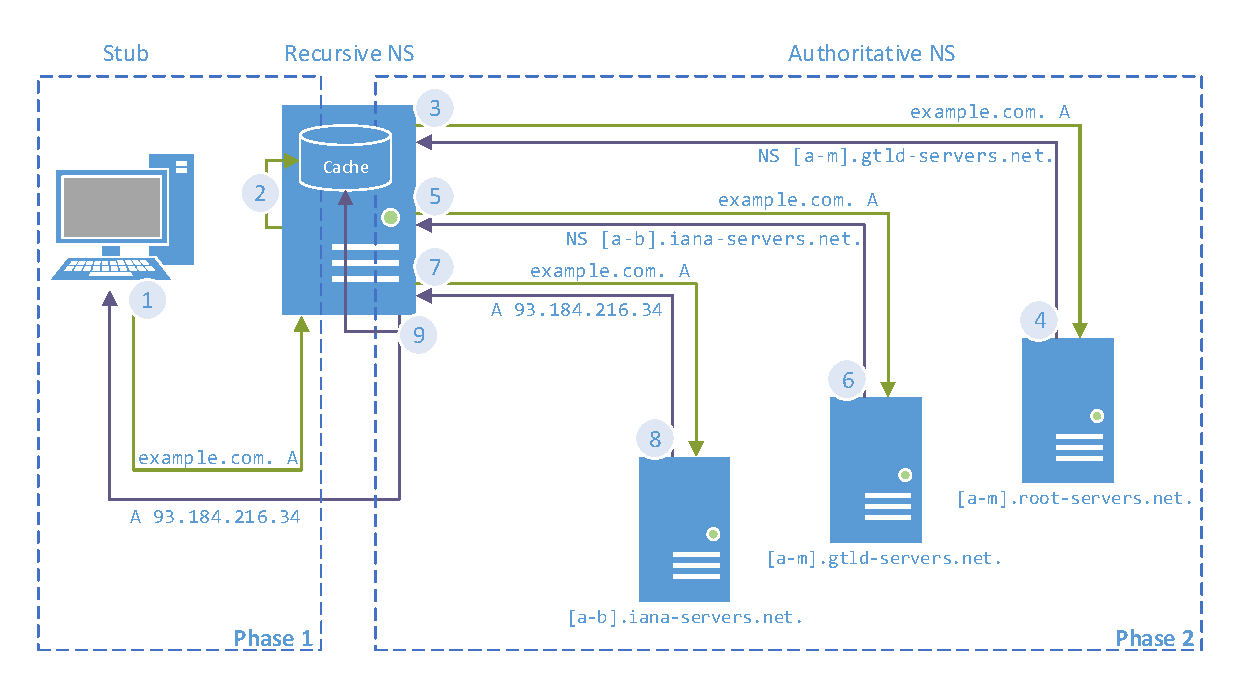
\includegraphics[width=\textwidth]{DNS_Resolution}
    \caption{Der schrittweise dargestellte Auflösungsprozess des Namen \texttt{example.com} über DNS. Der zeitliche Ablauf wird über die nummerierten Markierungen angezeigt.}
    \label{img:dnsresolution}
\end{figure}

\section{DNS Security}
\label{sec:dnssecurity}
Obwohl oder gerade weil DNS eines der grundlegendsten Services im Internet darstellt, wurde bei der Spezifikation des Netzwerkprotokolls bewusst auf eine Authentifizierung verzichtet. Dies ist auf die Idee einer öffentlich zugänglichen, globalen Datenbank, nach dem Vorbild eines globalen Telefonregisters, zurückzuführen. Die Datenbasis der Namensauflösung wurde somit als frei öffentlich zugänglich definiert. Abgesehen davon stammt das Protokoll aus einer Zeit in der modernen Schutzzielen wie Sicherheit und Vertraulichkeit wenig Beachtung geschenkt wurde. Dies führt zu einer Vernachlässigung des Sicherheitsgedanken und hat sich über die Zeit zu einem ernstzunehmenden Problem entwickelt. Verschärfend kommt hinzu, dass kein allgemeiner Konsens über die Sicherheitsziele herrscht. Dies erschwert die Entwicklung einer Lösung und hat zu den unterschiedlichsten Ansätzen und Technologien geführt \cite{Grothoff2018}. Die übergeordneten Lösungskonzepte werden in Kapitel \ref{chap:solutions} näher behandelt.

\section{Resolver Position}
\label{sec:dnsresolverposition}
Der Aufbau der Client-nahen Infrastruktur spielt eine wichtige Rolle für die Sicherheit des Clients. Wie im Abschnitt \ref{sec:dnsresolution} beschrieben, wird vom Client ein Recursive Resolver benötigt um die eigentliche Auflösung der Namen durchzuführen. Die Lage dieser Komponente im Netzwerk ist dabei vor allem für Privacy ausschlaggebend. Es existieren insgesamt fünf mögliche Positionen die ein Recursive Resolver einnehmen kann\cite{VanHeugten2018} (siehe Abbildung \ref{img:dnsresolverposition}):

\paragraph{Local Recursive Resolver}
Ist der Recursive Resolver im Netzwerk des Clients positioniert und wird die selbe öffentliche IP-Adresse zur externen Kommunikation benützt, spricht man von einem \textit{Local Recursive Resolver}. Da dieser in den meisten Fällen unter der Kontrolle des Benutzers steht und auch nicht von Dritten überwacht wird, ist es unbedenklich, dass Anfrage und Client-IP einfach ausgelesen werden können. Da für die gesamte internet-gerichtete Kommunikation, inklusive des rekursiven Auflöseprozesses, die selbe Adresse verwendet wird, ist es für Betreiber von Zwischenstellen einfach eine Verbindung zwischen Anfrage und User herzustellen\cite{Shulman2014}.

\paragraph{Private Recursive Resolver}
Unter \textit{Private Recursive Resolver} können alle Resolver zusammengefasst werden, die zwar unter der Kontrolle der nutzenden Personen stehen, aber nicht die selbe Adresse für die Kommunikation verwendet. Da die autoritativen DNS-Server von der Resolver-Adresse aus angesprochen werden, ist keine Verknüpfung zur Client-Adresse mehr möglich. Dies hilft der Privacy jedoch nur, wenn die Adresse des Servers nicht trotzdem einer einzelnen Person zugeordnet werden kann.

\paragraph{ISP Recursive Resolver}
Die Mehrheit der Nutzenden im privaten oder einzelunternehmerischen Umfeld verwenden den Resolver ihres \ac{ISP}. Diese \textit{ISP Recursive Resolver} werden von den Internetanbietern zur Verfügung gestellt, um eine grundlegende Internetkonnektivität anbieten zu können. Diese Server sind in den meisten Fällen im Netzwerk des ISP positioniert und haben daher oft bessere Latenzzeiten als andere, über das Internet erreichbare, Resolver. Diese Resolver werden oft für das überwachen von Kundenaktivitäten und einspeisen von Werbeseiten verwendet \cite{Weaver2011}, was grundsätzlich gegen den Gedanken der Privacy verstößt.

\paragraph{Public Recursive Resolver}
Sogenannte \textit{Public Recursive Resolver} sind über ihre freie Zugänglichkeit definiert und haben je nach Fokus des Anbieters verschiedenste Regelungen was Privacy betrifft \cite{Prince2018}\cite{Quad92018}. Wird nun ein Anbieter mit speziellem Fokus auf Sicherheit und Vertraulichkeit gewählt, kann ein akzeptabler Grad an Privacy erreicht werden. Voraussetzung dafür ist die Sicherung der Übertragung zwischen Stub-Resolver und Recursive Resolver. Einige Projekte bieten dafür Unterstützung spezielle Netzwerkprotokolle, die diesen Zweck erfüllen sollen (siehe dazu Kapitel \ref{chap:technologies}). Resolver die speziellen, selbst auferlegten Vorschriften zur Verbesserung der Informationssicherheit folgen, werden auch als \textit{Trusted Resolver} bezeichnet, wobei diese öffentlich (public) oder nur mit Authentifizierung (private) zugänglich sein können.

\paragraph{Local-Loopback Resolver}
Eine Sonderform stellt der \textbf{Local-Loopback Resolver} dar. Dieser wird direkt auf dem Client-Rechner installiert und ist nur für Programme auf eben diesem Host erreichbar. Dies führt zu dem Umstand, dass der Stub-Resolver keine für das umliegende Netzwerk sichtbare Kommunikation mehr durchführt. Der Installierte Resolver löst die Anfragen dann entweder rekursiv über das Netzwerk auf oder fungiert als Forwarding Resolver (siehe Abschnitt \ref{sec:dnsserver}) und verhält sich somit wie ein Stub-Resolver.

\begin{figure}[htbp]
    \centering
    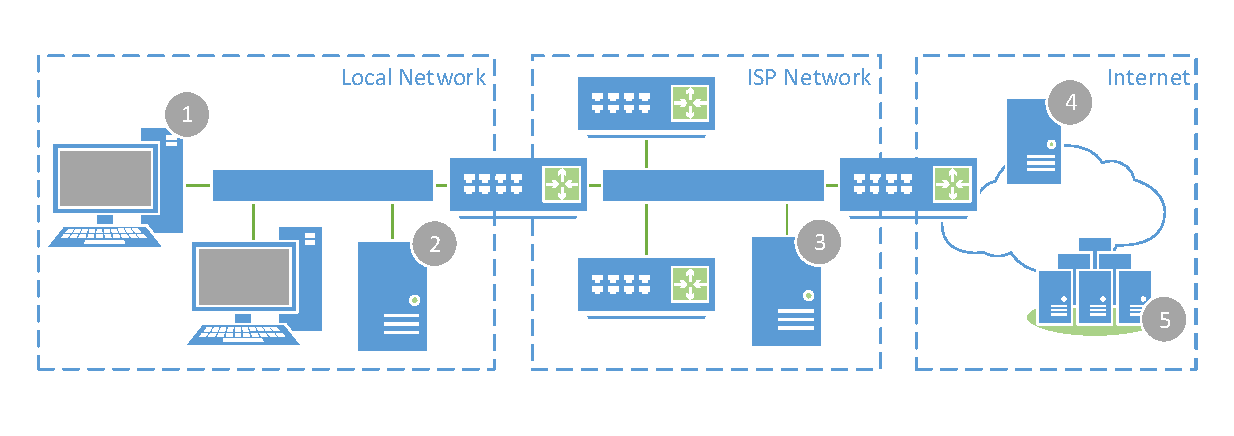
\includegraphics[width=\textwidth,trim={0 1cm 0 0.5cm},clip]{DNS_ResolverPosition}
    \caption{Zeigt die möglichen Positionen eines DNS-Resolvers. (1) Local-Loopback Resolver, (2) Local Recursive Resolver, (3) ISP Recursive Resolver, (4) Private Recursive Resolver, (5) Public Resolver}
    \label{img:dnsresolverposition}
\end{figure}


\chapter{Bekannte Probleme}
\label{chap:threads}

Das DNS als Gesamtsystem, sowie das ursprünglich spezifizierte Netzwerkprotokoll weisen einige Schwächen auf. Diese werden, angelehnt an die Schutzziele der Informationssicherheit (siehe Kapitel \ref{chap:itsecurity}), zu folgenden drei Problembeschreibungen zusammengefasst.   

\section{Fehlende Integritäts- und Authentizitätsprüfung}
\label{sec:thread-auth}

Wie in den Anfängen des \ac{WWW} und dessen Transportprotokoll \ac{HTTP} ist auch bei der Konzeptionierung der DNS Protokolls keine Rücksicht auf Sicherheitsaspekte wie Integrität, Authentizität und Vertraulichkeit genommen worden. Da DNS nach RFC1035\cite{rfc1035} auf jede Form von Authentifizierung verzichtet, ist ein Prüfen der Identität der jeweiligen Gegenstelle, sowie der eigentlichen Nutzdaten, nicht vorgesehen. Dies birgt eine hohe Anfälligkeit auf Angriffe die Anfragen und Antworten gezielt verändern. Des weiteren besteht keine Möglichkeit die Quellenauthentizität der RR zu prüfen. Damit können Angreifer gefälschte Einträge in die DNS Datenbank einbringen und so die Adresse bestimmter Servicenamen gezielt verändern. Diese Umleitung kann dann als Basis für umfangreiche Angriffe genutzt werden.

\section{Fehlender Schutz der Vertraulichkeit}
\label{sec:thread-priv}

Die DNS Sicherheitsvorfälle vergangener Jahre hat DNS-Privacy, als lange vernachlässigtes Thema, wieder ins Rampenlicht gerückt\cite{Greenwald2013}\cite{turkybbc2017}\cite{turkywp2018}. Die \ac{IETF} behandelt dieses Thema in der Arbeitsgruppe DPRIVE, welche sich ausschließlich mit DNS Privacy beschäftigt. Die 2013 veröffentlichten RFC6973 \textit{Privacy Considerations for Internet Protocols}\cite{rfc6973} bildet indem das Fundament für die aktive Förderung von vertraulicher Kommunikation im Internet. Für DNS wurde die darauf aufbauenden RFC7626 \textit{DNS Privacy Considerations}\cite{rfc7626} erstellt, welche die Relevanz von DNS Privacy klar darlegt. Im Speziellen wird auf die notwendige Unterscheidung zwischen der freien Zugänglichkeit der DNS Daten an sich und die Öffentlichkeit der Anfragen aufmerksam gemacht. Darüber hinaus existiert kein Schutz der Vertraulichkeit der Übertragung, dies macht Unberechtigten das mitlesen der Kommunikation möglich.

\section{Angreifbarkeit der Verfügbarkeit}
\label{sec:thread-dosamp}

DNS ist seit Jahren das meist angegriffene Internet-Service weltweit und befindet sich darüber hinaus als Trägertechnologie von DoS-Attacken auf Platz 1 \cite{Alcoy2017}. Das Fehlen eines Handshakes beim Verbindungsaufbau und die schlechte Zurückverfolgbarkeit machen DNS, neben dem \ac{NTP}, zur beliebtesten Verstärkungsmethoden für DoS-Angriffe. Da DNS-Server in den meisten Fällen von anderen DNS-Servern angegriffen werden, bedroht diese Anfälligkeit die Verfügbarkeit des Systems selbst, sowie anderer Systeme im Internet \cite{Kambourakis2008}.

\chapter{Angriffe}
\label{chap:attacks}
Um die Möglichkeiten potenzieller Angreifer und damit die möglichen Mitigation-Verfahren besser verstehen zu können werden nachfolgend die gängigsten Angriffe auf DNS beschrieben. Dabei wird spezieller Fokus auf für Clients relevante Gefahren gelegt. Angriffe die weder Vertraulichkeit, noch Integrität oder Verfügbarkeit des Clients gefährden werden bewusst nicht behandelt.

\section{DNS Sniffing}
\label{sec:attacks-dnssniffing}
Als Sniffing-Angriffe werden alle Arten von Angriffen bezeichnet die es ermöglichen Nachrichten zwischen mindestens 2 Parteien zu beobachten, mitzulesen und/oder mitzuhören\cite{CAPEC157}. In Hinblick auf DNS hat dies eine spezielle Bedeutung da es, aufgrund des fehlenden Schutz der Vertraulichkeit, ermöglicht, alle Informationen der Anfragen und Antworten einzusehen. Somit ist das Kommunikationsverhalten der Opfergeräte leicht nachzuvollziehen, was weiter Angriffe erheblich erleichtern kann. Das Aufzeichnen des DNS-Verkehrs lässt außerdem umfangreiche Schlussfolgerungen auf das Kommunikationsverhalten des Opfers zu. Darüber hinaus kann so auch die Transaktions-ID zusammen mit dem Ausgangsport erfahren werden, was die Voraussetzung für eine Spoofing-Attacke (siehe \ref{sec:attacks-dnsspoofing}) darstellt. 

\section{DNS Spoofing}
\label{sec:attacks-dnsspoofing}
\begin{wrapfigure}{r}{0.5\textwidth}
    \begin{center}
        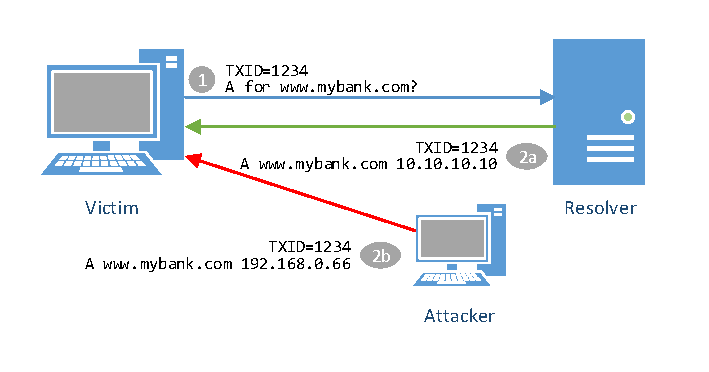
\includegraphics[width=0.48\textwidth,trim={8mm 8mm 8mm 8mm},clip]{DNS_Spoofing}
    \end{center}
    \caption{Darstellung einer klassischen DNS Spoofing Attacke.}
    \label{img:dnsspoofing}
\end{wrapfigure}

Spoofing Angriffe, auch \textit{Identity Spoofing} genannt, über die Aktion des ``zielgerichteten Glaubhaft machen einer gefälschten Identität'' definiert\cite{CAPEC151}. Es ist einem Angreifer dadurch möglich, dem Opfer falsche Informationen mitzuteilen, die als glaubwürdig und richtig behandelt werden. Im Fall von DNS spricht man von DNS Spoofing, was dieses simple Konzept auf einfache Art ausnützt.

Das DNS Netzwerkprotokoll verlässt sich beim prüfen der Authentizität der Antworten nun einerseits auf das Transportprotokoll (meistens UDP) und eine 16-bit \ac{TXID} \cite{rfc1035}. Gelingt es einem Angreifer nun sowohl das ausgehende Port, als auch die \ac{TXID} in Erfahrung zu bringen, ist es einfach möglich eine gefälschte, glaubwürdige Antwort zu generieren (siehe Abb. \ref{img:dnsspoofing}). Kommt diese nun vor der echten Antwort beim Client an oder wird sogar vom Angreifer ganz abgefangen, kann dem Opfer jede beliebige Antwort glaubhaft gemacht werden.

\subsection{DNS Cache Poisoning}
DNS Spoofing ermöglicht es auch den DNS-Cache eines Zielrechners aktiv zu Manipulieren. Angriffe die Einträge in Caches von Opfern verändern, werden allgemein als \textit{Cache Poisoning}-Attacken bezeichnet\cite{CAPEC141}. \textit{DNS Cache Poisoning} bietet somit die Möglichkeit, gezielt gefälschte Einträge in die Caches von Servern einzubringen\cite{CAPEC142}. Dies ermöglicht es einem Angreifer Verbindungen zu bestimmten Zieldomänen umzuleiten oder stillzulegen. Wie in Abb. \ref{img:dnscachepoisoning} zu sehen ist, wird für eine erfolgreiche Attacke kein Zugriff auf das Netzwerk des Opfers benötigt. Nachdem der Client die Anfrage an seinen Resolver abgesetzt hat (1), wird die Adresse über den rekursive Auflöse-Prozess ermittelt (2,3,4,5a). Ein Angreifer sendet nun Antworten mit der gefälschten Absenderadresse des autoritativen Nameservers an den Resolver (5b). Diese werden vom Resolver akzeptiert, sollte sie die richtige \ac{TXID} enthalten und zeitlich vor der echten Antwort ankommen. Aufgrund der geringen Entropie der \ac{TXID} (16-bit) ist das simple Erraten dieser ID zwar aufwendig aber durchführbar \cite{Son2010}. Wird die gefälschte Antwort vom Server nicht akzeptiert, erhält der Client die echte Antwort (6a). Gelingt jedoch das einbringen der falschen Antwort, sendet der Resolver die gefälschte Adresse zurück (6b). Je nach erhaltener Antwort, wählt der Host des Opfers den richtigen (7a) oder gefälschten (7b) Webserver als Ziel der Verbindung.    

\begin{figure}[htbp]
    \centering
    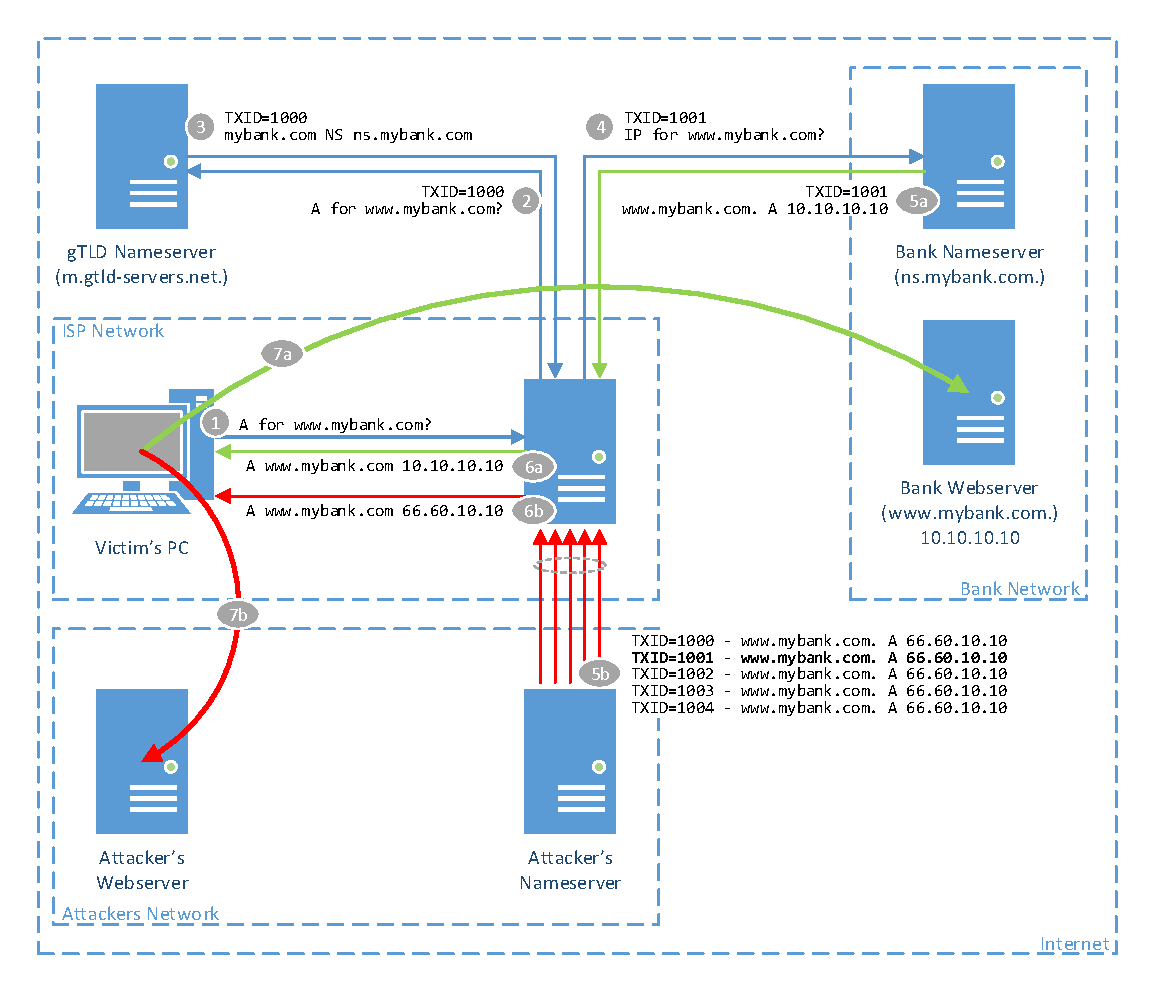
\includegraphics[width=0.8\textwidth]{DNS_CachePoisoning}
    \caption{Darstellung des Ablaufs einer DNS Cache-Poisoning Attacke}
    \label{img:dnscachepoisoning}
\end{figure}

\subsection{Kaminsky Angriff}
Eine viel gefährlichere Variante der Attacke ist 2008 vom amerikanischen Sicherheitsexperte Dan Kaminsky entwickelt worden\cite{Son2010}. In Abbildung \ref{img:dnskaminsky} wird gezeigt, wie es möglich ist, den Aufwand und die notwendige Zeit des Cache Poisoning massiv zu reduzieren. Dafür wird die Tatsache ausgenützt, dass die meisten Ziel-Resolver auch vom Angreifer erreichbar sind. Wird nun eine Anfrage zum Auflösen einer nicht existenten Unterdomäne der Zieldomäne an den Resolver gestellt (1) beginnt dieser mit der normalen Auflösung (2,3,4,5a). Da die Domäne nicht vorhanden ist, kann sie auch nicht in den Cache aufgenommen werden. Unterdessen sendet der Angreifer, wie im normalen Cache Poisoning auch, gefälschte Antworten an den Resolver (5b). Diese enthalten neben der Auskunft, dass die Domäne nicht existiert, einen zusätzlichen Eintrag der den Resolver über einen neuen Nameserver Eintrag informiert. Dieser gefälschter Eintrag enthält die Adresse eines Nameservers unter der Kontrolle des Angreifers. Ab diesem Zeitpunkt werden alle Anfragen an die Ziel-Domäne zum Nameserver des Angreifers weiterleiten. Dies stellt die effektive Übernahme der gesamten Domäne dar.

\begin{figure}[!hb]
    \centering
    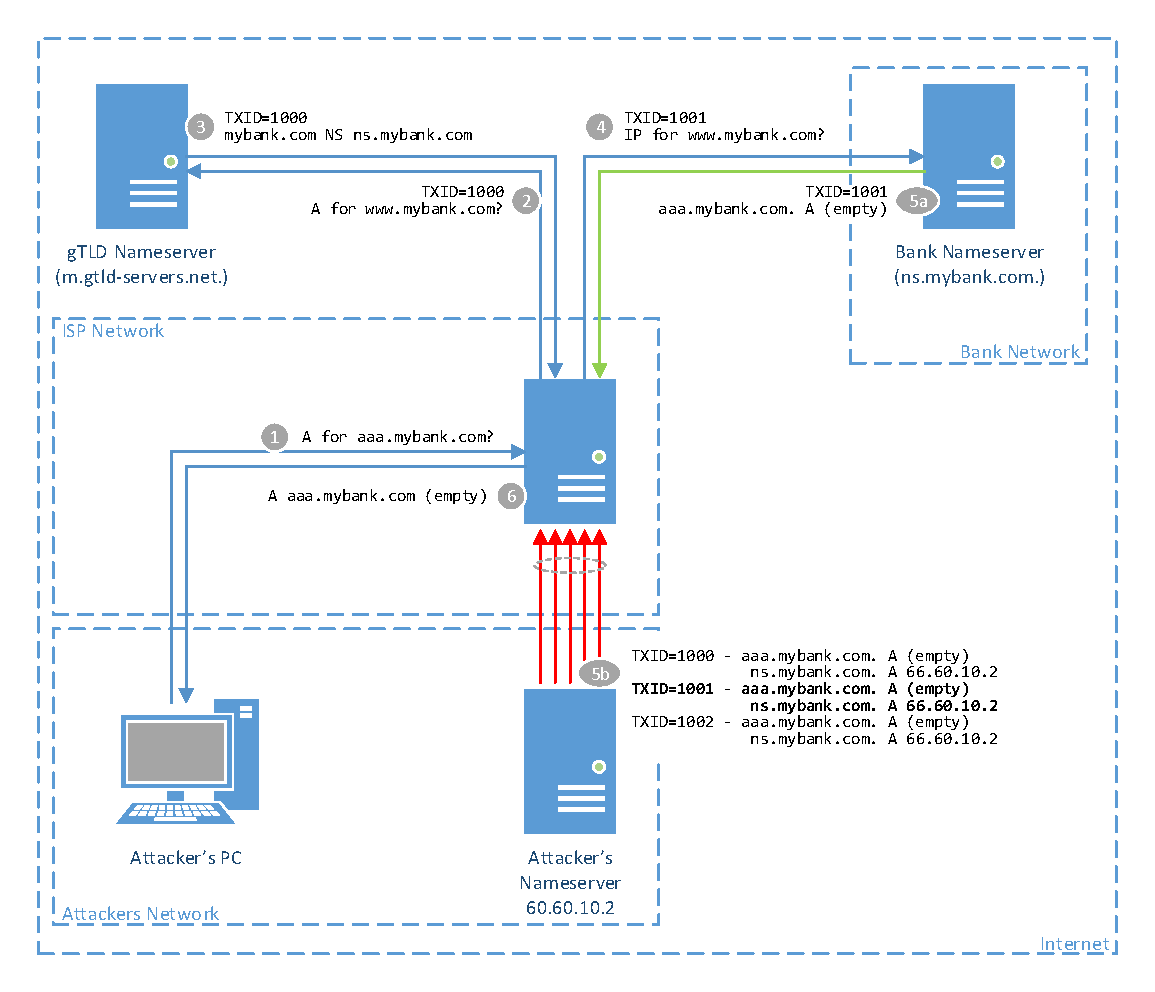
\includegraphics[width=0.8\textwidth]{DNS_Kaminsky}
    \caption{Schematische Darstellung des Ablaufs einer Kaminsky-Attacke}
    \label{img:dnskaminsky}
\end{figure}

Der Vorteil dieses Angriffs besteht in seiner beliebigen Wiederholbarkeit, da der eigentliche Eintrag nicht gecacht wird. Da der Auflöse-Prozess außerdem bewusst vom Angreifer initiiert wird, ist das korrekte Timing einfacher, die Attacke dadurch zuverlässiger.

\subsection{DNS Fragmentation Angriff}
Die Paketgröße der Vermittlungsschicht (OSI Layer 3) in Computernetzwerken ist limitiert, da die darunterliegende Sicherungsschicht (OSI Layer 2) nur Frames bis zu einer bestimmten Größe übertragen kann. Der limitierende Wert wird \ac{MTU} genannt und liegt in Ethernet-Netzwerken üblicherweise bei 1500 Bytes. Aufgrund dieser Beschränkung müssen Datagramme höherer Schichten, welche die MTU überschreiten, auf mehrere Unterpakete aufgeteilt werden. Dieser Vorgang wird als \textit{Fragmentierung} bezeichnet und kann für eine spezielle DNS Spoofing Attacke ausgenützt werden.

Bei DNS Spoofing muss der Angreifer die DNS \ac{TXID} (16-bit) erraten oder kennen. Nutzt man nun den Umstand der Fragmentierung, kann diese Unbekannte gegen einen andere, die IP-Fragment-Identification (IP-ID; 16-bit) getauscht werden. Der Vorteil dabei besteht in der besseren Vorhersagbarkeit dieser IP-ID da sie ausschließlich vom antwortenden Server gewählt wird. Dies macht es für einen Angreifer einfach den Auswahlalgorithmus des Ziels genau zu studieren. Paart man diese Schwachstelle nun mit den Techniken der anderen Angriffe, erhält man eine überaus effektive Möglichkeit DNS Caches zu manipulieren \cite{Herzberg2013}.

\section{Man-In-The-Middle Angriff}
\label{sec:attack-mitm}
Wie viele ältere Protokolle ist auch DNS von einer starken Anfälligkeit gegen sogenannte \ac{MITM} Attacken betroffen. Diese Art des Angriffs zeichnet sich durch den Umstand aus, dass sich der Angreifer unbemerkt zwischen zwei Kommunikationsteilnehmer Positionieren kann \cite{CAPEC94}. Aufgrund seiner vermittelnden Position ist er in der Lage die Kommunikation zwischen den Teilnehmern komplett zu Kontrollieren. Sollte er sich zwischen Endgerät und Recursive Resolver befinden, kann jede DNS-Interaktion nach belieben manipuliert werden. Solle es dem Angreifer gelingen, sich vor einem autoritativem DNS-Server zu stellen, können alle Anfragen und Antworten an die von diesem Server bereitgestellten Domänen, manipuliert werden. 

Da dieser Angriff derartig mächtig ist, bieten sich jedoch oft effektivere Wege um die Kontrolle über die Ziele auszuweiten. Die genauen Angriffswege und Möglichkeiten der Ausnutzung werden von Conti, Dragoni und Lesyk \cite{Conti2016} ausführlich beschrieben und würden den Rahmen dieser Arbeit sprengen.

\section{Denial-Of-Service Angriff}
\label{sec:attacks-dos}
\ac{DoS} Attacken  zielen darauf ab die Nutzung bestimmter Dienstleistungen, Funktionen oder Geräte zu verhindern \cite{BSIG040}. Durch einen solchen Angriff auf den verwendeten Resolver oder relevante, autoritative DNS-Servern können kritischen Unternehmensdienste kurzfristig außer Betrieb genommen werden. In den meisten Fällen wird für die Angriffe auf DNS die DNS-Infrastruktur selbst herangezogen. Ist es bei klassischen \ac{DoS} Attacken noch einfach die sendenden Hosts über Firewalls oder Routing stillzulegen, so kann das blockieren von DNS-Servern unvorhergesehene Auswirkungen auf die Funktionsweise des gesamten DNS haben\cite{Kambourakis2008}. 

\subsection{\ac{DoS}-Amplification Angriff}
\label{sec:attack-dosamp}
\begin{wrapfigure}{r}{0.35\textwidth}
    \begin{center}
        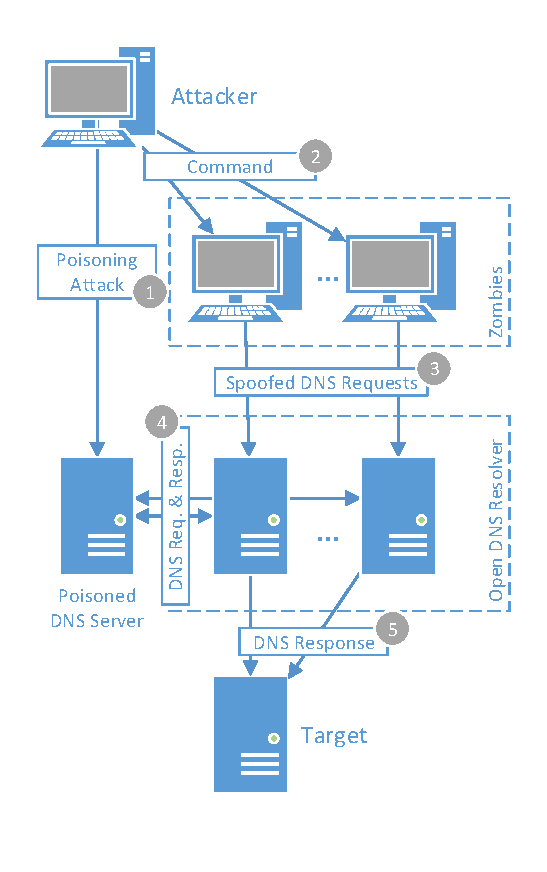
\includegraphics[width=0.33\textwidth,trim={5mm 10mm 5mm 10mm},clip]{DNS_DoS}
    \end{center}
    \caption{Darstellung eines \ac{DoS} Angriffs mit DNS-Amplification.}
    \label{img:dnsdos}
\end{wrapfigure}

Die Nutzbarkeit von DNS als Verstärker (Amplifier) von \ac{DoS} Attacken ist schon länger bekannt und wurde auch schon früher als Problem erkannt \cite{ICANN2006}. Das Problem liegt hier an dem eingesetztem Transportprotokoll UDP zusammen mit dem Umstand, dass DNS keinerlei Authentifizierung des Clients verlangt. Sendet ein Angreifer nun ein Paket mit gefälschter Absenderadresse an einen DNS-Resolver so wird dieser eine entsprechende Antwort an den vermeintlichen Absender schicken. Wird nun eine große Anzahl an solchen Anfragen an mehrere Resolver gestellt, kann dies schnell zu einer teilweisen oder vollständigen Sättigung der Bandbreite des gewählten Ziels führen. Die Kommunikationsfähigkeit des Opfers kann somit erheblich beeinträchtigt werden, was zu einem \ac{DoS} führen kann. 

Verschärfend kommt hinzu, dass der übliche maximale Verstärkungsfaktor von 12,8 mittels \ac{DNSSEC} (siehe \ref{sec:tec-dnssec}) auf durchschnittlich 47,2 erhöht werden kann. Dies ist auf die mit \ac{DNSSEC} eingeführte Erweiterung EDNS0 zurückzuführen, die es ermöglicht größere Antwortpakete anzufragen. Es konnte gezeigt werden, dass beim Nutzen aller Möglichkeiten einen maximalen Verstärkungsfaktor von 102,4 möglich ist\cite{VanRijswijk-Deij2014}. Mit dieser Verstärkung wäre ein Angreifer mit 100Mbit/s Bandbreite dazu in der Lage ca. 10Gbit/s Traffic zu generieren.

\paragraph{}
Effektive Angriffe machen sich die beschriebene hohen Verstärkungsrate und geringen Transparenz des Systems zu nutze \cite{Kambourakis2008}. Ein Angriff kann nun wie folgt ablaufen (siehe Abb. \ref{img:dnsdos}):
\begin{enumerate}[topsep=0pt,itemsep=-1ex,partopsep=1ex,parsep=1ex]
    \item Ein Angreifer bringt über Cache Poisoning einen speziellen RR (Amplifying Record) in einen Zielserver ein, der eine maximal große Antwort erzeigt.
    \item Einem zuvor gebildeter Bot-Netz wird nun das Kommando zum Anfragen dieses speziellen RR erteilt. 
    \item Es wird dabei ein DNS-Request mit gefälschter Absende-Adresse des Ziel an verschiedene offene Resolver gesendet.
    \item Die Resolver fragen nun den Manipulierten Eintrag am und erhalten eine große Antwort.
    \item Da die Absende-Adresse gefälscht wurde, werden die Antworten an das Opfer gesendet und nehmen aufgrund ihrer Größe und Anzahl einen großen Anteil der Bandbreite ein. 
\end{enumerate}
Werden nun stetig neue Anfragen gestellt und eine ausreichend hohe Anzahl an Zombie-Rechnern bzw. Resolvern verwendet, kann die gesamte Bandbreite des Opfers saturiert werden. Dies stellt den als \ac{DoS} bezeichneten Zustand dar.

\section{DNS Rebinding}
\label{sec:attack-dnsrebind}
Eine weniger bekannte Art die Schwachstellen von DNS auszunutzen ist das sogenannte \textit{DNS Rebinding}. Ziel des Angriffs besteht im Überwinden der als \textit{Access Within Same Origin Policy} genannte Sicherheits-Technik moderner Browser. Diese verbietet es Scripts einer Webseite auf Inhalte zuzugreifen die nicht unter dem selben Hostnamen erreichbar sind. Es können zwar Ausnahmen definiert werden, da dies jedoch am Ziel passieren muss, besteht dadurch keine Gefahr. Die Schwachstelle besteht nun im Fakt, dass DNS-Einträge mit sehr geringer TTL gesetzt werden können. Es wird dadurch möglich die Adresse eines Namens während der Ausführung eines Scripts zu verändern\cite{Jackson2009}. Das ermöglicht den folgenden Ablauf.

\begin{enumerate}
    \item Das Opfer wird vom Angreifer auf eine von ihm kontrolliere Website gelockt. Der Nameserver des Angreifers vergibt für den DNS-Eintrag des Webservers eine sehr geringe TTL.
    \item Der Browser des Opfers führt die auf der Webseite eingebunden Scripts aus. Gleichzeitig läuft die TTL des gecachten Eintrags aus, was den Resolver zu einer erneuten Auflösung bewegt. Bei dieser wird nun vom Nameserver des Angreifers die Adresse eines Ziels zurück geliefert.
    \item Nach diesem \textit{Rebinding} des Hostnamen kann das laufende Script über den eigenen Namen auf die Ressourcen der Adresse des Ziels zugreifen. Dies erlaubt dem Script z.B. Zugriffe auf netzinterne Ressourcen wie Administrationsoberflächen oder ermöglicht das Scannen des LANs. Außerdem wird damit der Browser des Opfers für andere Angriffe, wie \ac{DoS} Attacken, nutzbar.   
\end{enumerate}

Auch wenn es viele Gegenmaßnahmen in aktuellen Browsern gibt und einige der anfälligen Komponenten (Java Applets, Flash, etc.) an Verbreitung verlieren, besteht besonders durch die zunehmende Verbreitung von IoT-Geräten eine akute Bedrohung durch diesen Angriffsweg\cite{Dorsey2018}. 

\section{BitSquatting}
Eine weitere, ausgefallene Angriffsmöglichkeit bietet das sogenannte \textit{BitSquatting}. Bei diesem Angriff werden zufällige Fehler im Hauptspeicher von Geräten ohne fehlererkennende Speichermodule ausgenützt. Es konnte gezeigt werden, dass es durch solche Fehler zum stellen fehlerhafter Anfragen an potenziell existente Domänen kommen kann\cite{Dinaburg2011}. Dieser Effekt kann nun bewusst ausgenutzt werden, indem eine große Anzahl an Domänen registriert werden, deren Name sich nur um ein Bit von viel besuchten Domänen unterscheidet (siehe Listing \ref{lst:bitquatting}). 
Da es in diesem Fall zu stellen falschen Anfragen kommt, gibt es auch keine Möglichkeit sich auf Protokoll- bzw. System-Ebene zu schützen. Die einzige effektive Lösung stellt der Einsatz von \textit{Error-correcting code memory} Hardware dar.  
\begin{lstlisting}[caption={Drei mögliche BitSquatting-Domänen für die Zieldomäne \texttt{amazon.com}}, label={lst:bitquatting}]
amazon.com = 61   6d   61 7a   6f   6e 2e 63 6f 6d
           ... 01101101 ... 01101111 ... 
aeazon.com = 61   65   61 7a   6f   6e 2e 63 6f 6d  
           ... 01100101 ...
                   ^
a-azon.com = 61   e2   61 7a   6f   6e 2e 63 6f 6d 
           ... 00101101 ...
                ^
amazgn.com = 61   6d   61 7a   67   6e 2e 63 6f 6d
                        ... 01100111 ...
                                ^
\end{lstlisting}

\section{Übersicht}
Gruppiert man nun die oben gezeigten Angriffe nach den in Kapitel \ref{chap:threads} beschriebenen Schwächen erhält man die in Abbildung \ref{img:attacks-summary} dargestellte Zuordnung. DNS Rebinding und BitSquatting wurden dabei als spezielle Attacke gesondert betrachtet.

\begin{figure}[!hb]
    \centering
    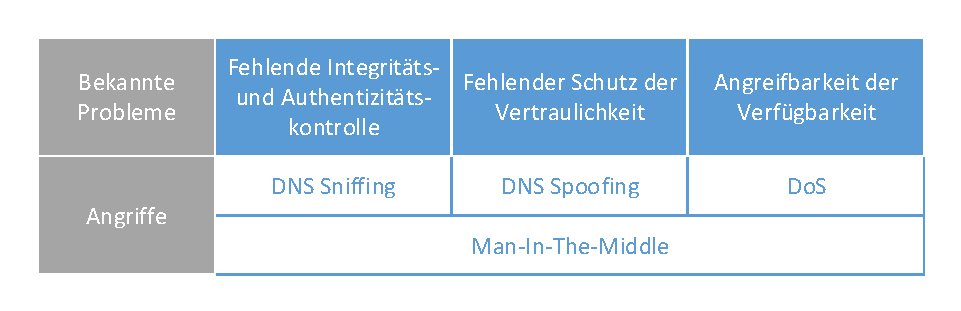
\includegraphics[width=\textwidth]{Overview_Attacks}
    \caption{Übersicht des Bezugs zwischen den vorgestellten Sicherheits-Problemen und den Attacken die diese ausnutzen.}
    \label{img:attacks-summary}
\end{figure}



\chapter{Lösungsvorschläge}
\label{chap:solutions}
Aufgrund der in den vorherigen Kapiteln beschriebenen Problemen und Angriffen können insgesamt sechs Lösungsvorschläge erstellt werden. Diese sind als Empfehlungen zu verstehenden und werden bereits von verschiedenen, existierenden Technologien erfüllt. Auf diese wird im Kapitel \ref{chap:technologies} genauer eingegangen.

\section{Authentizität der Records}
\label{sec:solution-recordauth}
Wie in Kapitel \ref{sec:thread-auth} beschrieben wurde, ist die Authentizität der \ac{RR} ein zentrales Problem in DNS. Eine einfache Lösung stellt der Einsatz kryptografischer Signaturen dar. Mit diesen können alle Einträge bei der Erstellung signiert und dadurch geschützt werden. Werden die Signaturen bei der Abfrage mit übertragen, können sie vom Client validiert werden. Dies macht die Sicherstellung der Integrität und Authentizität der empfangenen Einträge möglich. Werden die Zonendateien nur bei Änderungen signiert ist die Zone außerdem vor ungewollter Veränderung zu schützen. Das notwendige Vertrauen, in die für die Signaturen verwendeten Schlüssel, kann hierbei auf verschiedenste Wege erreicht werden (siehe Kapitel \ref{sec:trust}).

\section{Authentizität der autoritativen Server}
Neben der Authentizität der RR selbst, spielt zusätzlich die Authentizität der autoritativen DNS-Server eine wichtige Rolle. Einige der angeführten Angriffe, nutzen den Umstand, dass Resolver keine Möglichkeit besitzt die Identität der Gegenstellen zu prüfen. 

Eine Lösung besteht in der Signatur der Records (siehe \ref{sec:solution-recordauth}), ist jedoch einfacher möglich: Formal genügt es eine kurzlebige, verschlüsselte Sitzung zwischen Resolver und autoritativen Server zu etablieren. Dies kann über klassischen hybriden Verschlüsselungsverfahren erreicht werden. Ein Problem stellt dabei der Aufbau einer zuverlässigen Vertrauensstellung dar (siehe Abschnitt \ref{sec:tec-dnscurve}).

\section{Authentizität des Resolvers}
In Kapitel \ref{sec:thread-auth} wurde erwähnt, dass es im DNS-Netzwerkprotokoll keine Möglichkeit gibt die Authentizität der Gegenstelle, im Speziellen des Resolvers, zu prüfen. Abhilfe für dieses Problem schafft einerseits das zuvor besprochene kryptografische Signieren der Einträge. Dieser Schutz scheitert hingegen oft an der praktischen Umsetzung, da dieser durch einen MITM-Angriff (siehe Abschnitt \ref{sec:attack-mitm}) überwindbar ist \cite{Bau2010}. 

Eine mögliche Lösung dieses Problem stellt das Einführen eines Authentifizierungsverfahren dar. In den meisten Fällen wird dafür eine auf asymmetrische Kryptografie basierende Methode eingesetzt. Wir schon in Abschnitt \ref{sec:trust} erwähnt, gibt es verschiedene Möglichkeiten das notwendige Vertrauen zu einem gegebenen Schlüssel herzustellen. Nach der Authentifizierung kann die Authentizität der einzelnen Nachrichten über Signaturen geprüft werden.

\section{Vertraulichkeit der Verbindung}
Wie in Abschnitt \ref{sec:thread-priv} dargelegt ist DNS-Privacy zu einem wichtigen Thema geworden. Die nachhaltige Lösung zur Sicherstellung der Vertraulichkeit ist, wie damals bei HTTP, der Einsatz einer geeigneten Transportverschlüsselungstechnologie. Auf welcher Ebene diese Stattfindet ist dafür grundsätzlich nicht relevant. Der Einsatz von etablierten Technologien wie TLS liegt dennoch nahe, obwohl für DNS zudem alternative Lösungen entwickelt wurden. 

\section{Trennen von Adresse und Anfrage}
\label{sec:goals-sourceanon}
Um die sensiblen Verbindungsdaten zu schützen ist es wichtig, die Anonymität der anfragenden Person zu wahren. Konkreter sollen Adressen, die mit der entschlüsselten Anfrage in Verbindung steht, nicht auf die anfragende Person zurückführbar sein. Durch den Einsatz von rekursiven Resolvern wird diese Kombination aus Adresse und Anfrage zwar vor den autoritativen DNS-Servern verborgen, verschiebt das Problem dabei lediglich auf den Resolver. 

Die Lösung besteht in der Trennung von Adresse des Clients und dessen entschlüsselter Anfrage bzw. Antwort. Um dies zu ermöglichen ist es notwendig, dass der erste, vom Client direkt angesprochene Server, nicht in der Lage ist die echte DNS-Anfrage oder Antwort zu entschlüsseln. Die Aufgabe dieses Servers besteht darin, die wahre Adresse des Clients zu verbergen und die Anfrage von einer anderen Adresse aus an einen Resolver weiterzuleiten. Der Resolver muss dann in der Lage sein, die Anfrage zu entschlüsseln, ist aber nicht mehr in Kenntnis über die echte Adresse des Fragestellers. Damit ist das problematische Tupel aus Adresse und Daten aufgelöst, was zur Verbesserung der Privacy beiträgt \cite{Schmitt2018}.

\section{Verbindungbehaftete Protokolle einsetzen}
\label{sec:goals-trafficamp}
Wie in Abschnitt \ref{sec:attack-dosamp} beschrieben, wird DNS selbst als Verstärker (Traffic Amplification; DoS Amplification Attack) für DoS-Attacken eingesetzt. Es ist daher zum Schutz anderer Internet-Services essenziell, das DNS und dessen Implementierungen vor dieser Art der Ausnützung zu schützen.

Die einfachste Möglichkeit einer Lösung besteht im Ablösen des Verbindungslosen UDP zugunsten eines Verbindungsorientierten Protokolls wie TCP. Der notwendige Verbindungsaufbau könnte im Falle eines klassischen IP-Spoofings nicht abgeschlossen werden, was das Stellen einer Anfrage verhindern würde. Damit wäre DNS nicht mehr als Verstärker nutzbar. Dieser Vorteil ist direkt mit dem Nachteil verbunden, dass der Verbindungsaufbau viel Zeit in Anspruch nimmt und zusätzliche Ressourcen auf dem Server bindet. Wie festgestellten werden konnte, ist die Auswirkung auf die Performance in den meisten Fällen jedoch stark überschätzt \cite{Zhu2015}.

Neben TCP können Protokolle wie DTLS, trotz UDP Transportprotokoll, eingesetzt werden. DTLS baut eine Sitzung auf, was die Möglichkeit zum Einsatz als Verstärker ebenfalls erschweren würde, da der Server erst nach erfolgreichem Handshake Anfragen akzeptiert \cite{rfc6347}. 


\chapter{Technische Umsetzungen}
\label{chap:technologies}

\section{DNSSEC}
\label{sec:tec-dnssec}
DNSSEC, als eine Sammlung an IETF-Spezifikationen, erweitert DNS mit dem Ziel die Integrität und Authentizität der Ressourceneinträge sicherzustellen \cite{Arends2005}. Dies wird über die kryptografische Signatur der Einträge erreicht. Die Signaturen werden pro RRSet in eigenen RR vom Typ RRSIG gespeichert und den Antworten beigefügt. Zur Validierung wird eine Chain-Of-Trust (siehe Abschnitt \ref{sec:trust}) genützt, die ihren Ankerpunkt in einem \ac{DNSSEC}-Root-Key besitzt, welcher von der ICANN veröffentlicht wird. Der Umstand, dass die ICANN somit als alleinige Kontrollinstanz (Single-Point-Of-Trust) fungiert, wird teils als Verletzung des Grundgedankens eines verteilten, unabhängigen Internets verstanden \cite{Finch2014}.
Abgesehen davon findet die Erweiterung, aufgrund der langen Entwicklungszeit, der (verglichen zum DNS-Protokoll) hohen Komplexität und dem erhöhtem administrativem Aufwand, nur wenig Anklang. Seit der finalen Veröffentlichung 2005 konnten zwar 90 Prozent der TLD-Betreibenden zum Signieren ihrer Zonen bewegt werden, die Verbreitung signierter SLDs ist mit ca. 4 Prozent jedoch zu gering um Maßgeblich zur Sicherheit des globalen DNS beizutragen \cite{DCCommunications2018}. Zusätzlich wurde das Schutzziel der Vertraulichkeit bewusst unbehandelt gelassen. Wie in Abschnitt \ref{sec:thread-priv} beschrieben, ist der Bedarf nach einer vertraulichen Möglichkeit zur Auflösung von Namen im Internet stark angestiegen. Betrachtet man zusätzlich den Umstand, dass das \ac{DNSSEC}s Netzwerkprotokoll noch stärker als reines DNS, für \ac{DoS}-Amplification genützt werden kann, ist klar, warum diese Spezifikationssammlung so wenig positive Resonanz erhält \cite{Antic2014}.

\section{DNSCurve}
\label{sec:tec-dnscurve}
Aufgrund der schlechten Akzeptanz von \ac{DNSSEC} veröffentlichte der US-amerikanische Kryptograf \ac{DJB} eine eigene Lösung namens DNSCurve. Diese dient zur Sicherstellung einer vertraulichen und authentischen Kommunikation zwischen rekursiv auflösendem Server und den autoritativen Servern. Diese baut auf dem, von \ac{DJB} entwickelten, elliptische Kurven-Kryptosystem Curve25519 auf. DNSCurve verwendet, im Gegensatz zu \ac{DNSSEC}, welches RSA einsetzt, \ac{ECC} für asymmetrische Operationen. Außerdem wird der, ebenfalls selbst entwickelte, Poly1305 \ac{MAC} für die Verschlüsselung und Echtheitsprüfung der Nachrichten eingesetzt. 

Der Einsatz von \ac{ECC} sorgt, im Vergleich zu RSA, für eine signifikante Verbesserung der Performance bei der Schlüsselaushandlung. Da weit kürzere Schlüssel bei gleichbleibender Sicherheit eingesetzt werden können, werden außerdem Probleme mit übergroßen Paketen verhindert \cite{Gupta2002}. Der in RFC7905 \cite{rfc7905} spezifizierten Poly1305 Algorithmus ist ebenfalls auf Geschwindigkeit unter Einhaltung der Sicherheitsansprüche optimiert \cite{Bernstein2005}. Somit war DNSCurve bei seiner Veröffentlichung 2009 \ac{DNSSEC} überlegen. Da der höhere Leistungsanspruch der Validierung bis heute ein starkes Argument gegen den Einsatz von \ac{DNSSEC} dargestellt, wurde DNSCurve trotz der ungewöhnlichen Algorithmen positiv aufgenommen \cite{Henry2013}. Dies Überrascht, da DNSCurve, wie D. Kaminsky feststellt, ein konzeptionelles Problem im Bereich des \textit{Trust Establishment}-Prozesses aufweist \cite{Kaminsky2011}. 

Das Protokoll verlässt sich beim Auffinden der öffentlichen Schlüssel auf einen speziellen NS-Eintrag, jenen zur Ziel-DNS-Domäne. Da DNSCurve ohne Erweiterungen des DNS-Protokolls auskommt, wird dieser Eintrag lediglich durch dessen spezielles Format aufgefunden. Darüber hinaus wird der Schlüssel in den NS-Eintrag selbst kodiert. Ein Angreifer in einer aktiven MITM Position (siehe \ref{sec:attack-mitm}) könnte somit, durch simples Umschreiben des Eintrags, eine Kommunikation über DNSCrypt unterbinden. Selbst wenn kein Fallback zur Klartextkommunikation erfolgt, besteht noch immer die Möglichkeit, ein eigenes Schlüsselpaar zu generieren und den öffentlichen Schlüssel des Ziels gegen diesen zu tauschen. In der Spezifikation scheint zwar die Möglichkeit zum Aufbau einer CoT auf, da eine zentrale Vertrauensinstanz bewusst fehlt, wird diese von Kaminsky als \textit{ineffektiv} bezeichnet, da sie laut ihm keine zufriedenstellende Lösung des Problems bringt. Es ist somit fraglich, ob DNSCurve  Vertraulichkeit und Authentizität von DNS sicherstellen kann.  

\section{DNSCrypt}
Zusätzlich zu DNSCurve und \ac{DNSSEC} wurde 2011 das Netzwerkprotokoll DNSCrypt entwickelt. Dieses ähnelt DNSCurve im grundlegenden Aufbau, da es die Algorithmen Curve25519 und Poly1305 verwendet und das standardkonforme DNS Netzwerkprotokoll für die Kommunikation einsetzt. Der größte Unterschied liegt darin, dass DNSCrypt die Kommunikation zwischen Stub-Resolver und rekursivem DNS Server schützt. Um dies zu erreichen werden kurzlebige Zertifikate eingesetzt, welche zur Verschlüsselung der Anfragen und Validierung der Antworten eingesetzt werden. Diese Zertifikate sind mit einem langlebigen Schlüssel signiert, wobei der öffentliche Schlüssel von jedem Client explizit in eine Liste an vertrauenswürdigen Schlüsseln aufgenommen werden muss \cite{Denis2016}. Dies umgeht zwar die konzeptionelle Schwäche von DNSCrypt, ist jedoch ohne entsprechende Unterstützungsmethoden nicht praktikabel. Eine in manchen Implementierungen verwendete Lösung nach dem \ac{TOFU} Prinzip wird als nicht zuverlässig erachtet \cite{Wendlandt2008}. 

Somit stellt DNSCrypt, ähnlich wie DNSCurve, zwar eine sichere  Möglichkeit zum Übertragen von DNS-Anfragen und Antworten an den auflösenden DNS Server dar, vernachlässigt jedoch ebenfalls das zentrale Thema des \textit{Schlüsselmanagements}. Eine Möglichkeit zum Umgehen dieser Schwäche stellt das Nutzen der öffentlichen Browser-PKI CoT oder das Etablieren eines direkten Trusts dar. Wird das genutzte Zertifikat zum Beispiel manuell geprüft und explizit eingespielt, kann dieses von einem möglichen Angreifer nicht mehr modifiziert werden. Werden diese Wege genutzt, kann das System als ausreichend sicher angesehen werden.

\section{DNS-over-TCP}
Eine minimalistische Lösung für die DoS und Traffic-Amplification Problematik (siehe Abschnitt \ref{sec:attacks-dos}) ist der Einsatz eines verbindungsorientierten Protokolls. Hier bietet sich TCP an, da es bereits als mögliches Transportprotokoll im ursprünglichen Standard festgelegt wurde \cite{rfc1035}. Obwohl der als \ac{T-DNS} bezeichnete Vorschlag schon früh aufkam, wurde ihm lange keine Beachtung geschenkt. Der Zeitaufwand für das Aufbauen einer Verbindung, zusammen mit dem erhöhten Ressourcenaufwand auf der Serverseite, wurde als finales Gegenargument gegen den Einsatz von \ac{T-DNS} verwendet. Seit 2014 mehren sich jedoch die Argumente gegen dieses Dogma. Es konnte klar festgestellt werden, dass moderne Systeme durchaus in der Lage sind, diese erhöhten Ansprüche zu erfüllen \cite{Zhu2015}. 

\section{DNS-over-TLS}
\label{sec:tec-dot}
Den Umstand der fehlenden Authentizität und Vertraulichkeit hat DNS mit vielen älteren Netzwerkprotokollen gemein. Ein weiteres,  im \ac{WWW} sehr verbreitetes Protokolle ist das \ac{HTTP}. Als Lösung für HTTP wurde das \ac{TLS} Protokoll festgelegt, welches das meist genutzte Transportverschlüsselungsprotokoll der TCP/IP-Suite darstellt. Es liegt also nahe, die Sicherheitsschwäche von DNS ebenfalls mit TLS als Transportprotokoll zu beheben.

Angestoßen durch die früheren Arbeiten zu \ac{T-DNS} wurde das Anbieten von \ac{DoT} im IETF Dokumenten RFC7858 \cite{rfc7858} und RFC8310 \cite{Dickinson2018} spezifiziert. Es ist seit 2016 als sichere Transportmethode zwischen zwei DNS-Endpunkten akzeptiert. Die Aufgabe der Authentifizierung wurde auf das TLS Protokoll übertragen und folgt damit denselben Mechanismen, welche schon von HTTPS bekannt sind. Die über ein X509 Zertifikat authentisierende Gegenstelle wird im Zuge des TLS-Handshake, über vorinstallierte Zertifikate von Zertifizierungsstellen, authentifiziert (siehe \ref{sec:trust}).

\section{DNS-over-HTTPS}
Einen mit DoT vergleichbaren Ansatz wählt die im IETF Draft zu \ac{DoH} beschriebene Technologie \cite{Mcmanus2018}. Diese Technik nützt HTTPS statt TLS als Trägerprotokoll und ermöglicht damit nativen Web Applikation die Auflösung von DNS Anfragen. Der Entwurf sieht zusätzlich die Möglichkeit einer \textit{Server Push} Funktion vor, welche es \ac{DoH}-DNS-Servers erlaubt, von sich aus Pakete an Clients zu senden. Es wird argumentiert, dass so der Auflösungsprozess beschleunigt werden kann, da zusätzlich zur eigentlichen Anfrage, andere zugehörige Einträge mit gesendet werden können. Diese müssen dann nicht nochmals angefragt werden, sondern sind schon im Cache des Resolvers geladen. Zusätzlich soll es möglich sein, die bestehende HTTP-Caching-Infrastruktur für DoH-Anfragen mitzubenützen. Die Funktionsweise im Hinblick auf Vertraulichkeit und Authentizität unterscheidet sich nicht von DoT und ist somit grundlegend valide. 

\section{EncDNS und Oblivious DNS}
\label{tec:encdns-odns}
Wie in Abschnitt \ref{sec:goals-sourceanon} angesprochen, besteht aus Sicht der Vertraulichkeit das Problem, dass der gewählte Recursive-Resolver einfach Zugriff auf die Kombination von Client-Adresse und angefragte Zieladresse besitzt. Spezielle Relevanz erhält das Thema, da Trusted Resolver aktuell einen starken Zulauf erhalten und so immer mehr dieser Daten binden.

EncDNS \cite{Herrmann2014} und \ac{ODNS}\cite{Schmitt2018} sind beide ähnliche Technologien, die als Ziel die Auftrennung dieser Kombination anstreben. Um die Verschleierung der Client-Adresse zu erreichen wird ein jeweils eigener Stub-Resolver eingesetzt. Dieser erstellt DNS Anfragen mit einem speziell aufgebauten Anfragenamen. Die eigentliche DNS-Anfrage wird dabei verschlüsselt und als Präfix zu einer speziellen Domäne verpackt (z.B. \texttt{ax3kp5ao9v.EncDNS.com}). Der autoritative Server dieser Domäne muss entsprechend fähig sein, dieses Format zu verstehen. Dieser Aufbau veranlasst den Recursive-Resolver, die Anfrage normal abzuarbeiten, was diese schlussendlich zum autoritativen Server leitet. Dieser entschlüsselt die spezielle Anfrage und führt die eigentliche Auflösung durch. Danach wird die verschlüsselte Antwort formuliert und an den Resolver zurückgeschickt, welcher sie an den Client weitergibt.

Durch die Verschlüsselung ist es dem Recursive-Resolver nicht möglich, die echte Anfrage und Antwort zu lesen. Des Weiteren ist auch der autoritative DNS-Server nicht in Kenntnis über die echte Adresse des Clients. Somit wurde die Verknüpfung zwischen Client-Adresse und Anfrage gelöst.

Der Unterschied zwischen EncDNS und ODNS besteht in den eingesetzten Protokollen zur Verschlüsselung und zum Transport der Nachrichten. EncDNS ist stark von DNSCurve inspiriert und baut somit auf dieselben Algorithmen und Formaten auf. ODNS folgt zwar dem grundlegenden Konzept von EncDNS, legt den Fokus jedoch auf Performance und Verfügbarkeit. Diese Entscheidung spiegelt sich vor allem im Einsatz eines verteilten Key Distribution Mechanismus wider. Dieser erlaubt es dem System einen, für den Resolver, optimalen DNS-Server zu wählen ohne dasselbe Schlüsselpaar auf alle DNS-Server verteilen zu müssen. Als Algorithmen setzt ODNS AES für Sitzungsschlüssel und ECIES für den Schlüsseltransport ein.

Wie schon im Abschnitt \nameref{sec:tec-dnscurve} erwähnt, erben damit beide Systeme dieselbe Schwäche im Trust-Establishment Prozess. Ein Angreifer, der den kompletten Netzwerkverkehr des Opfers unter Kontrolle hat, könnte den initialen öffentlichen Schlüssel verändern und sich somit als Resolver oder EncDNS bzw. ODNS Server positionieren.

\section{Address-Obfuscation über NAT}
\label{sec:tec-nat}
Technologien wie EncDNS und \ac{ODNS} (sieht \ref{tec:encdns-odns}) verwenden das Kernkonzept der ``Trennung von Adresse und Anfrage'' zur Verbesserung der Privacy. Nimmt man etwas Abstand, so erkennt man, dass es sich um eine Variante des Reverse-Proxy-Konzepts handelt. Betrachtet man die in RCF1631 \cite{rfc1631} spezifizierte \ac{NAT} Technologie so findet man den Hinweis, dass diese zur Verbesserung der Privacy betragen könne. Dies folgt aus dem Umstand, dass NAT die Absenderadresse gegen die des NAT-Servers tauscht. Werden Anfragen verschiedener Clients durch einen NAT-Server zum Resolver geleitet, wird der Zusammenhang zwischen Anfrage und Adresse aufgehoben, solange die IP des NAT Servers keine 1:1-Relation zum Client zulässt. Die Vertraulichkeit der Anfrage gegenüber dem NAT-Server wird dabei durch die Transportverschlüsselung gewährleistet, wobei die Adresse gegenüber dem angesprochenen Resolver mittels NAT verborgen wird.

Als Alternative zu diesem Konzept kann der Einsatz eines VPN-Gateways genannte werden. Diese Technologien nutzen Verfahren, welche teils hohe Aufwände an Rechenleistung und Bandbreite mit sich bringen. Außerdem wird die Latenzzeit durch die längeren Wege und ineffizientes Routing massiv erhöht. Dies verschlechtert die Benutzbarkeit erheblich und ist daher nicht als alltagstauglicher Ersatz zu verstehen.      

\section{Übersicht}
In Abbildung \ref{img:technologies-summary} sind die beschriebenen Probleme (siehe \ref{chap:threads}), Lösungsmöglichkeiten (siehe \ref{chap:solutions}) und Technologien zueinander in Bezug gebracht.

\begin{figure}[!hb]
    \centering
    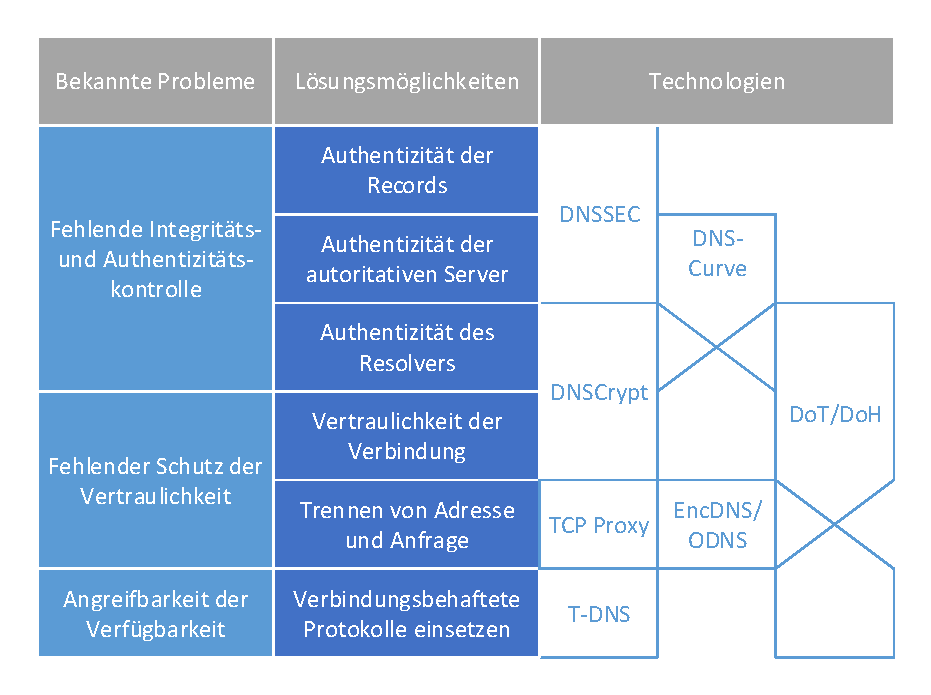
\includegraphics[width=0.7\textwidth]{Overview_Tecs}
    \caption{Darstellung des Bezugs zwischen DNS-Security Problemen, Lösungsmöglichkeiten und den bestehenden Technologien zur Umsetzung der Lösungen}
    \label{img:technologies-summary}
\end{figure}

\chapter{Implementierung}
\label{chap:implementation}

Um die in Kapitel \ref{chap:threads} beschriebenen Probleme zu mindern oder gar zu beheben, kann eine Auswahl an vorgestellten Technologien (siehe \ref{chap:technologies}) genutzt werden. Das Ziel ist dabei der Schutz einer kleinen Anzahl von Clients durch den Einsatz eines speziell konfigurierten lokalen, rekursiven Resolvers. Es ist dabei nicht sinnvoll alle anwendbaren Techniken einzusetzen, da jede mit Kosten in Performance einhergeht, wobei die Vorteile mancher Kombinationen redundant sind.

\section{Position und Resolver Typ}
Die möglichen Positionen und Betriebsarten eines Resolvers (siehe Abb. \ref{img:impl-resolverpositions}) wurden bereits im Abschnitt \ref{sec:dnsresolverposition} behandelt. Für die Auswahl wurden drei Kriterien betrachtet: Angreifbarkeit, Performance und Privacy.
\begin{figure}[hb]
    \centering
    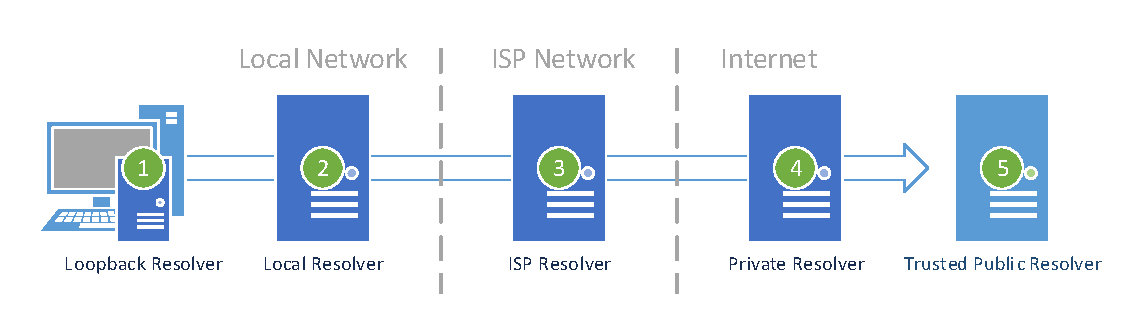
\includegraphics[width=\textwidth,trim={8mm 8mm 8mm 8mm},clip]{Impl_ResolverPositions}
    \caption{Stellt die möglichen Positionen eines Resolvers, aus Sicht des Clients, dar.}
    \label{img:impl-resolverpositions}
\end{figure}

\paragraph{Local-Loopback Resolver (1)}
Diese Position ist bei einem, auf die Verbindung zwischen Recursive Resolver und Stub-Resolver abgezielten, Angriff die sicherste. Werden Techniken wie DoT, DoH oder DNSCrypt im Forwarding Modus eingesetzt, kann darüber hinaus die Vertraulichkeit und Authentizität bis zum Recursive Resolver sichergestellt werden. Die Nachteile ist die fehlende Möglichkeit eines geteilten Caches, die erhöhte Ressourcenverbrauch am Client und der hohe Wartungsaufwand. Außerdem können keine Internet-Of-Things (IoT) Geräte bedient werden, da bei diesen eine Installation eines lokal laufenden Resolvers nicht möglich ist.

\paragraph{Local Network Resolver (2)}
Durch einen Resolver im Lokalen Netzwerk, besteht zwar die Gefahr von Angriffen auf Netzwerkebene, es wird jedoch der Einsatz eines gemeinsamen Caches möglich und eine hohe Geräte-Kompatibilität stakt verbessert. In kleinen, gut gesicherten Netzwerken kann dieses Angriffsszenario aufgrund des geringen Risikos in Kauf genommen werden. Angriffe von außen sind jedoch durchaus möglich und wahrscheinlich, sollte der Resolver nicht speziell geschützt werden.

\paragraph{ISP Resolver (3)}
Da, wie in Abschnitt \ref{sec:thread-priv} beschrieben, nicht auf die Verantwortlichkeit von ISPs oder staatlichen Institutionen vertraut werden sollte, ist das Nutzen eines ISP-Resolvers, vor allem in Hinblick auf Privacy, nicht zu empfehlen. Einzige Ausnahme stellt dabei der Einsatz von Technologien wir DNSCurve, EncDNS und ODNS dar, da diese eine Verschlüsselung der Anfragen durch den Resolver hindurch unterstützen. Aufgrund kurzer Laufwege und großen Caches sind diese Resolver in den meisten Fällen durchaus performant.

\paragraph{Private Resolver (4)}
Betreibt man seinen eigenen Resolver im Internet erhält man dadurch Kontrolle über die Privacy-Einstellungen des Resolvers. Abgesehen davon, setzt man sich damit jedoch allen möglichen Angriffen, nicht nur auf DNS, aus. Darüber hinaus sind die meisten Stub-Resolver nicht dazu in der Lage über sichere Protokolle mit dem Resolver zu kommunizieren. Abgesehen davon muss darauf geachtet werden, dass keine Zuordnung zwischen der Resolver-IP in einzelnen Personen hergestellt werden kann. Da diese Nachteile den Vorteilen stark überwiegen kann vom Einsatz eines eigener, privater Resolvers abgeraten werden.

\paragraph{Public Resolver (5)}
Der direkte Einsatz eines Trusted Public Resolvers hat viele Vorteile. Die Performance ist aufgrund guter Anbindungen, eines professionellen Betriebs und großen Caches meist gut. Viele Resolver haben spezielle Schutzmaßnahmen gegen Cache Poisoning- oder DoS-Attacken im Einsatz. Außerdem ist die Anonymität gegenüber autoritativen DNS-Servern, aufgrund der hohen Zahl an Users, als ausreichend anzusehen. Der einzige, schwerwiegende Nachteil besteht in der Gefahr von Privacy-Verletzungen durch den Betreiber des Dienstes. Hier ist entweder eine Abwägung zu treffen oder eine Lösung zur vollständigen Anonymisierung zu finden. 

\section{Technologie-Stack}
Zur Auswahl des Sets an Technologien (hier als ``Stack'' bezeichnet) wurde aufgrund der, am Ende des Kapitels \ref{chap:attacks} angeführten, Übersicht erstellt. Dabei wurde darauf geachtet, jede der unter \ref{chap:solutions} abgegebenen Empfehlungen gerecht zu werden. Um die Auswahl besser verstehen zu können, wird hier kurz auf jede einzelne der Techniken eingegangen.

\paragraph{DNSSEC}
DNSSEC stellt aktuell die einzige Möglichkeit zur Echtheitsprüfung von RRs selbst dar (siehe Abschnitt \ref{sec:tec-dnssec}). Das Abfragen und Validieren der \ac{DNSSEC} RRSig-Records ist somit Pflicht für jeden Resolver mit Sicherheitsfokus. Die Validierung kann an verschiedenen Stellen erfolgen. Da die Validierung aufgrund der kryptographischen Operationen durchaus ressourcenintensiv sein kann, ist es Sinnvoll diese Operation nicht auf jedem Client durchzuführen. Abgesehen davon fehlt vielen Stub-Resolvern die Möglichkeit zur selbstständigen Validierung. Wird ein Forwarding-Resolver eingesetzt, kommt es auf die Konfiguration und Implementierung an ob dieser eine Validierung durchführt oder sich auf den nachgeordneten Recursive Resolver verlässt. Kann dem rekursiven Resolver vertraut werden, ist die Verifizierung durch diesen, aus Effizienzgründen, zu bevorzugen.

\paragraph{DNS-over-TLS}
Wie in Abschnitt \ref{sec:tec-dot} beschrieben stellt DoT einen simplen Aufsatz zum klassischen DNS Netzwerkprotokoll dar. Für den Transport wird TLS über TCP auf Port 853 genutzt\cite{rfc7858}. Damit ist die Verbindung zwischen Resolver und Recursive Resolver geschützt. 

\paragraph{Address-Obfuscation über NAT}
Um auch die Vertraulichkeit der Anfragen erhalten zu können, kann zusätzlich der Zusammenhang zwischen der Client-Adresse und der Anfrage aufgelöst werden. Dies kann, wie schon in Abschnitt \ref{sec:tec-nat} erwähnt, durch den Einsatz eines NAT Servers erreicht werden. Zur Umsetzung kann nahezu jedes modernen Server-Betriebssystem herangezogen werden.

\section{Konzept}
Aus den beschriebenen Vor- und Nachteilen ergibt sich der Einsatz eines lokalen Forward-Resolver als optimaler Kompromiss aus Sicherheit, Kompatibilität und Performance. Der beschriebene Technologie-Stack ist in der Lage alle in Kapitel \ref{chap:solutions} vorgestellten Empfehlungen zu erfüllen. In Abbildung \ref{img:impl-architecture} wird der schematische Ablauf der Kommunikation gezeigt. Es werden dabei zusätzlich die Übergangsstellen der Verschlüsselung und Client-Identifizierbarkeit gezeigt.
\begin{figure}[hb]
    \centering
    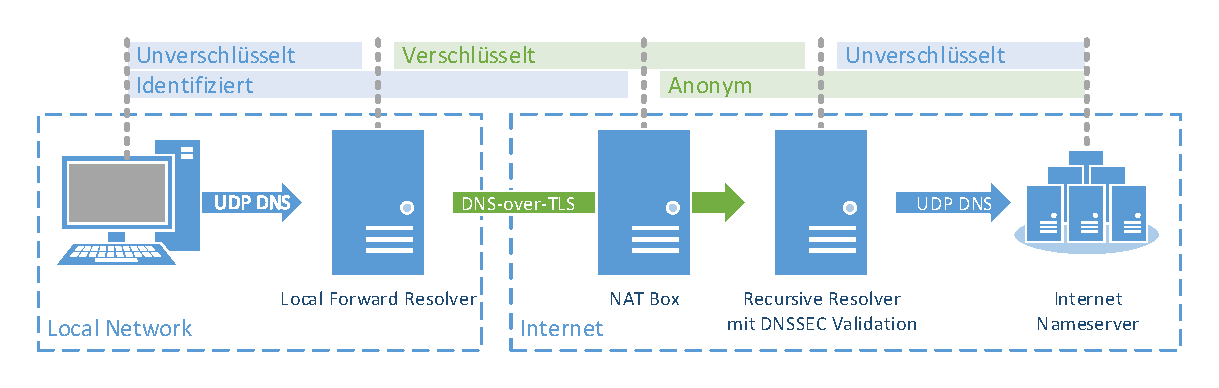
\includegraphics[width=\textwidth,trim={5mm 5mm 5mm 5mm},clip]{Impl_Architecture}
    \caption{Darstellung des schematischen Kommunikationsweg des Test-Aufbaus.}
    \label{img:impl-architecture}
\end{figure}

Um die Privacy der lokalen Clients und damit der Nutzenden zu wahren, wurde der Aufbau nach einem einfachen Grundkonzept entworfen: Entschlüsselte DNS-Nachrichten dürfen nur auf vom User direkt kontrollierten Komponenten mit der externen Internet-Adresse verknüpfbar sein. Dadurch wird verhindert, dass Betreiber der Transportnetzwerke oder der nachgeordneten DNS-Komponenten private Daten mit der Identität der Nutzenden verknüpfen.

Des weiteren wird durch DoT jede Form von Sniffing und Spoofing Attacken unmöglich gemacht. Da der Forwarding-Resolver selbst keine normalen DNS Anfragen von außerhalb des lokalen Netzwerks annimmt, ist der Resolver auch gegen DNS DoS Attacken durch externe Angreifer geschützt. Die \ac{DNSSEC} Validierung erfolgt je nach Implementation am lokalen Forward-Resolver oder am Public-Recursive-Resolver. Es ist damit selbst im Falle einer erfolgreichen Cache-Poisoning Attacke auf den Public Resolver nicht möglich RRs zu kompromittieren, die durch \ac{DNSSEC} Signaturen geschützt sind.

\section{Aufbau}
\label{sec:architecture}
Zu Validierung des Entwurfs wurde ein einfacher Testaufbau umgesetzt. Dieser verwendet Windows 10\footnote{Microsoft Windows Version 1803 (Build 17134.285)} als Test-Client-Betriebssystem und Fedora 28\footnote{Linux 4.17.19-200.fc28.x86\_64} als Betriebssystem des lokalen Resolvers. Der Local-Resolver selbst wurden zwecks Vergleichbarkeit mit zwei verschiedenen Software-Paketen umgesetzt: Unbound\footnote{Version 1.7.3 (kompiliert mit OpenSSL 1.1.0h-fips)} und Knot-Resolver\footnote{Version 2.4.1}. Als Trusted-Public-Resolver wurde das Quad9-Projekt gewählt da es DoT anbietet und einer zu befürwortende Privacy-Policy\cite{Quad9Privacy} folgt. Darüber hinaus werden Domänen, die in Zusammenhang mit Schadsoftware stehen, vom Quad9-Resolver automatisch geblockt. Dieses Feature kann zwar als Zensur verstanden werden, durch die aktuelle Bedrohung durch DNS unterstützte Malware \cite{Alcoy2017} und die strikt auf ``Phishing, Malware, and Exploit-Kits'' konzentrierte Sperrliste\cite{Quad9FAQ} kann die Bedrohung durch Zensur der durch Malware vorübergehend untergeordnet werden.   
\begin{wrapfigure}{r}{0.5\textwidth}
    \begin{center}
    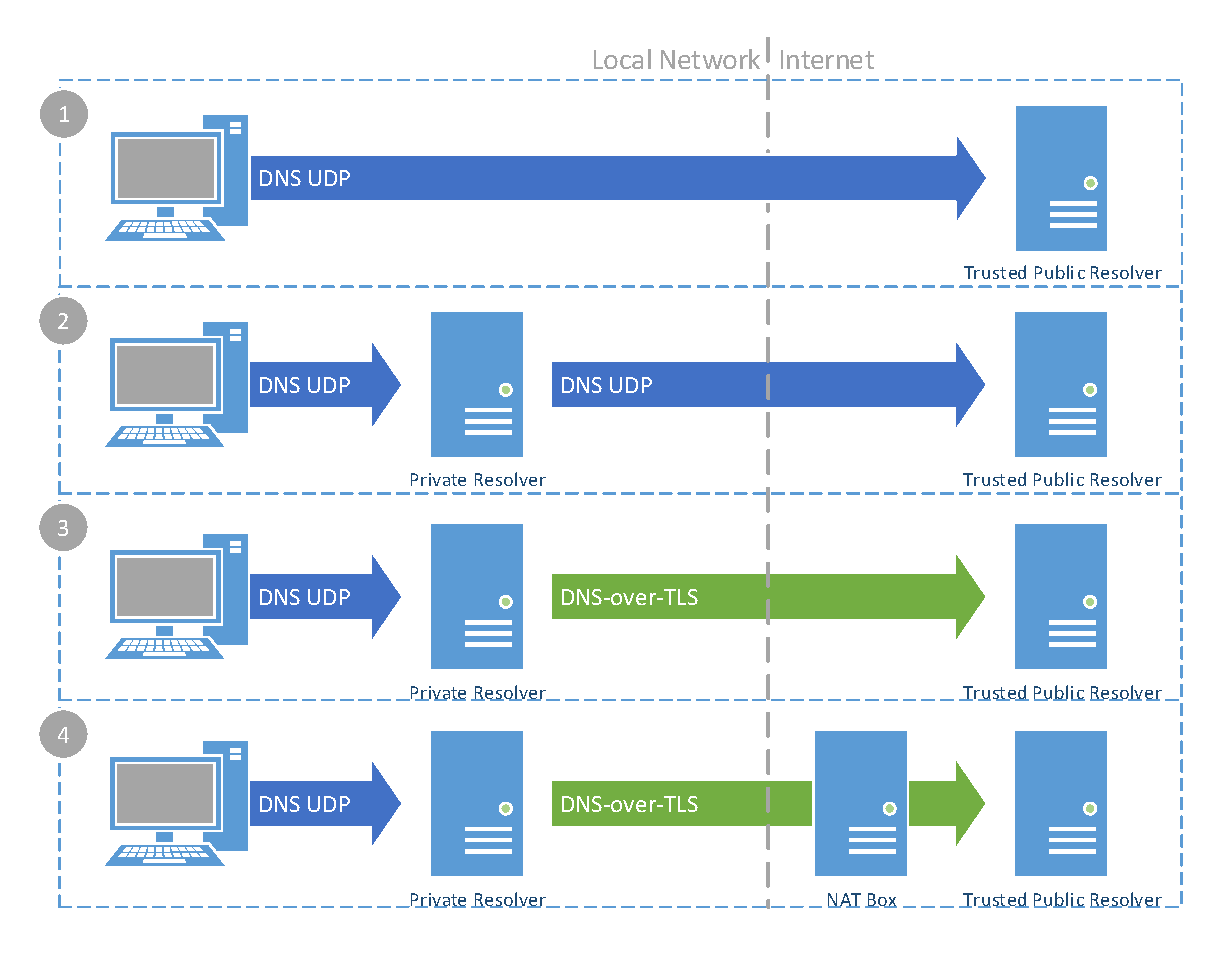
\includegraphics[width=0.48\textwidth,trim={5mm 8mm 5mm 8mm},clip]{Impl_Scenarios}
    \end{center}
    \caption{Darstellung der getesteten Szenarien}
    \label{img:impl-scenarios}
\end{wrapfigure}

Wie in Abbildung \ref{img:impl-scenarios} dargestellt wurden für den Performance- und Funktions-Test vier Szenarien gewählt. Dabei erfüllt nur Szenario 4 alle beschriebenen Schutzmechanismen, wobei Szenario 3 nur die Anonymität gegenüber des Public Resolver verletzt. Geht man von einem vertrauenswürdigen Anbieter dieses Resolvers aus, kann auf die Anonymisierung über den NAT-Server verzichtet werden. Wie man sieht, wird in jedem Fall von einem sicheren lokalen Netzwerk ausgegangen, mögliche Lösungen bei unsicheren Netzwerken wir in Kapitel \ref{chap:conclusion} diskutiert. 

\paragraph{Public-Resolver über UDP (1)}
Durch die direkte Verbindung zwischen Stub-Resolver und Public Resolver wird auf jegliche Vertraulichkeit der Übertragung verzichtet, da der in Windows integrierte Stub-Resolver keine Form der Verschlüsselung unterstützt. Abgesehen davon, ergibt sich durch die minimale Anzahl an Zwischenstellen eine optimale Latenzzeit, die sich positiv auf die gesamte Performance auswirkt.

\paragraph{Lokalen Forwarding-Resolver über UDP (2)}
In diesem Fall wird ein Forwarding-Resolver im lokalen Netzwerk installiert. Da dieser das klassische DNS-Netzwerkprotokoll zur Kommunikation mit dem Recursive-Resolver verwendet, ergibt sich noch kein Schutz der Vertraulichkeit. Mit einer restriktiven Konfiguration und verschiedenen, von der Implementation abhängigen, Sicherheitsfeatures können jedoch gewisse Arten von Spoofing-Attacken ausgeschlossen werden. Befindet sich eine Firewall an der Netzwerkkante so kann diese, durch den Einsatz eines lokalen Resolvers, sehr restriktiv Eingestellt werden. Dies verhindert direkte Angriffe auf Stub-Resolver von extern. Ein weiterer Vorteil besteht beim Einsatz von ``Knot-Resolver'' da dieser bestimmte DNS Rebinding Attacken (siehe \ref{sec:attack-dnsrebind}) abwehren kann, indem er interne IP-Adressen in Antworten verbietet\cite{KnotResolverDocRebinding}.

\paragraph{Lokaler Forwarding-Resolver mit DoT (3)}
Wird die Verbindung zum Recursive-Resolver nun durch ein Verschlüsselungsprotokoll wie DoT (siehe \ref{sec:tec-dot}) geschützt, ergibt sich ein klarer Vorteil: Es besteht eine sichere Verbindung zwischen dem Forwarding- und Recursive-Resolver, was Sniffing-, Spoofing-, sowie MITM-Attacken auf diesem Wege ausschließt. Durch den Einsatz von verbindungsorientierten Protokollen und Verschlüsselung werden jedoch der steigende Ressourcenverbrauch und höhere Latenzzeiten merkbar.

\paragraph{Lokaler Forwarding-Resolver mit DoT und NAT (4)}
Fügt man dem Aufbau nun einen NAT-Server (siehe \ref{sec:tec-nat}) hinzu, erhält man den Vorteil der Anonymität gegenüber des Recursive-Resolvers. Da dies der einzige Vorteil des Aufbaus darstellt, ist die dadurch einhergehende Erhöhung der Latenzzeit gegen den Schutzbedarf abzuwägen.

\section{Tests und Messungen}
\label{sec:measurements}
Die Kontrolle der unter \ref{sec:architecture} beschriebenen Varianten wurde nun mithilfe der Programme dig\footnote{Auf Ubuntu Subsystem for Windows10; DiG 9.10.3-P4-Ubuntu} sowie ``DNS Benchmark''\footnote{von Steve Gibson Version 1.3.6668.0} durchgeführt. Gemessen wird die gesamte benötigte Umlaufzeit (Round-Trip-Time; RTT) 100 ungecachter, zufälliger Einträgen. Die gewählten Konfigurationen der DNS-Server sind in \nameref{chap:appA} zu finden und wurden nach den offiziellen Dokumentationen und darin enthaltenen Sicherheitsempfehlungen erstellt. Als ``Hardware'' wurden 3 virtuelle Maschinen (1 vCPU, 1GB RAM) auf einem vom Test-Client unabhängigen Host genutzt. Um eine optimale Vergleichbarkeit der einzelnen Varianten zu erreichen wurden die Tests der Performance von einem Test-Client auf die 3 Server simultan durchgeführt. Dabei wurden in 2 unabhängigen Läufen alle unterschiedlichen Varianten einer Software getestet. In einem dritten Lauf wurde die direkte Performance von 25 offener DNS-Resolvern (siehe \ref{chap:appB}) getestet und die 10 besten zur Errechnung der direkten Vergleichswerte herangezogen. Für die Auswertungen wurden immer nur Werte von ungecachten Einträgen herangezogen, da nur diese eine Kommunikation mit dem Recursive-Resolver verlangen. Die Ergebnisse der Tests sind unter Kapitel \ref{chap:results} angeführt. 



\chapter{Ergebnisse}
\label{chap:results}

Die in Abschnitt \ref{sec:measurements} beschriebenen Messungen der Umlaufzeiten (Round-Trip-Times;RTT) verschiedener DNS-Anfragen ergaben die in Abbildung \ref{img:results-times} dargestellten Zeiten. Aus diesen Werten ergeben sich nun folgende Ergebnisse.

\paragraph{Performance Einbußen durch DoT}
Wie schon in Kapitel \ref{chap:implementation} näher ausgeführt, war ein Performanceverlust durch den Einsatz von DoT zu erwarten. Dieser schlägt sich speziell in den Minimalzeiten mit ca. 50-100\% Erhöhung nieder. Dies ist auf den notwendigen Verbindungsaufbau zurückzuführen. Diese Werte decken sich grob mit den früheren Messwerten aus der Arbeit von Zhu et al.\cite{Zhu2015} und zeichnen sogar ein etwas besseres Bild. Die durchschnittlichen RTTs der herkömmlichen DNS-Abfragen über UDP betragen dabei 105\,ms, wobei die über TLS mit 115-128\,ms um ca. 20\% erhöht sind.

\paragraph{Auswirkung des NAT-Servers}
Vergleicht man die Werde der Variante mit und ohne Anonymisierung mittels NAT, so erkennt man nur minimale Unterschiede. Je nach Implementation wurden Unterschiede von 5-11\,ms beobachtet, was bei einer Gesamtdauer von ca. 120\,ms ca. 5-9\% ausmacht. Da es zu den alternativen Anonymisierungstechnologien EncDNS und ODNS keine aktuellen Implementierungen gibt, kann dieser Zeitverlust mit keiner Alternative verglichen werden.

\begin{figure}[hb]
    \centering
    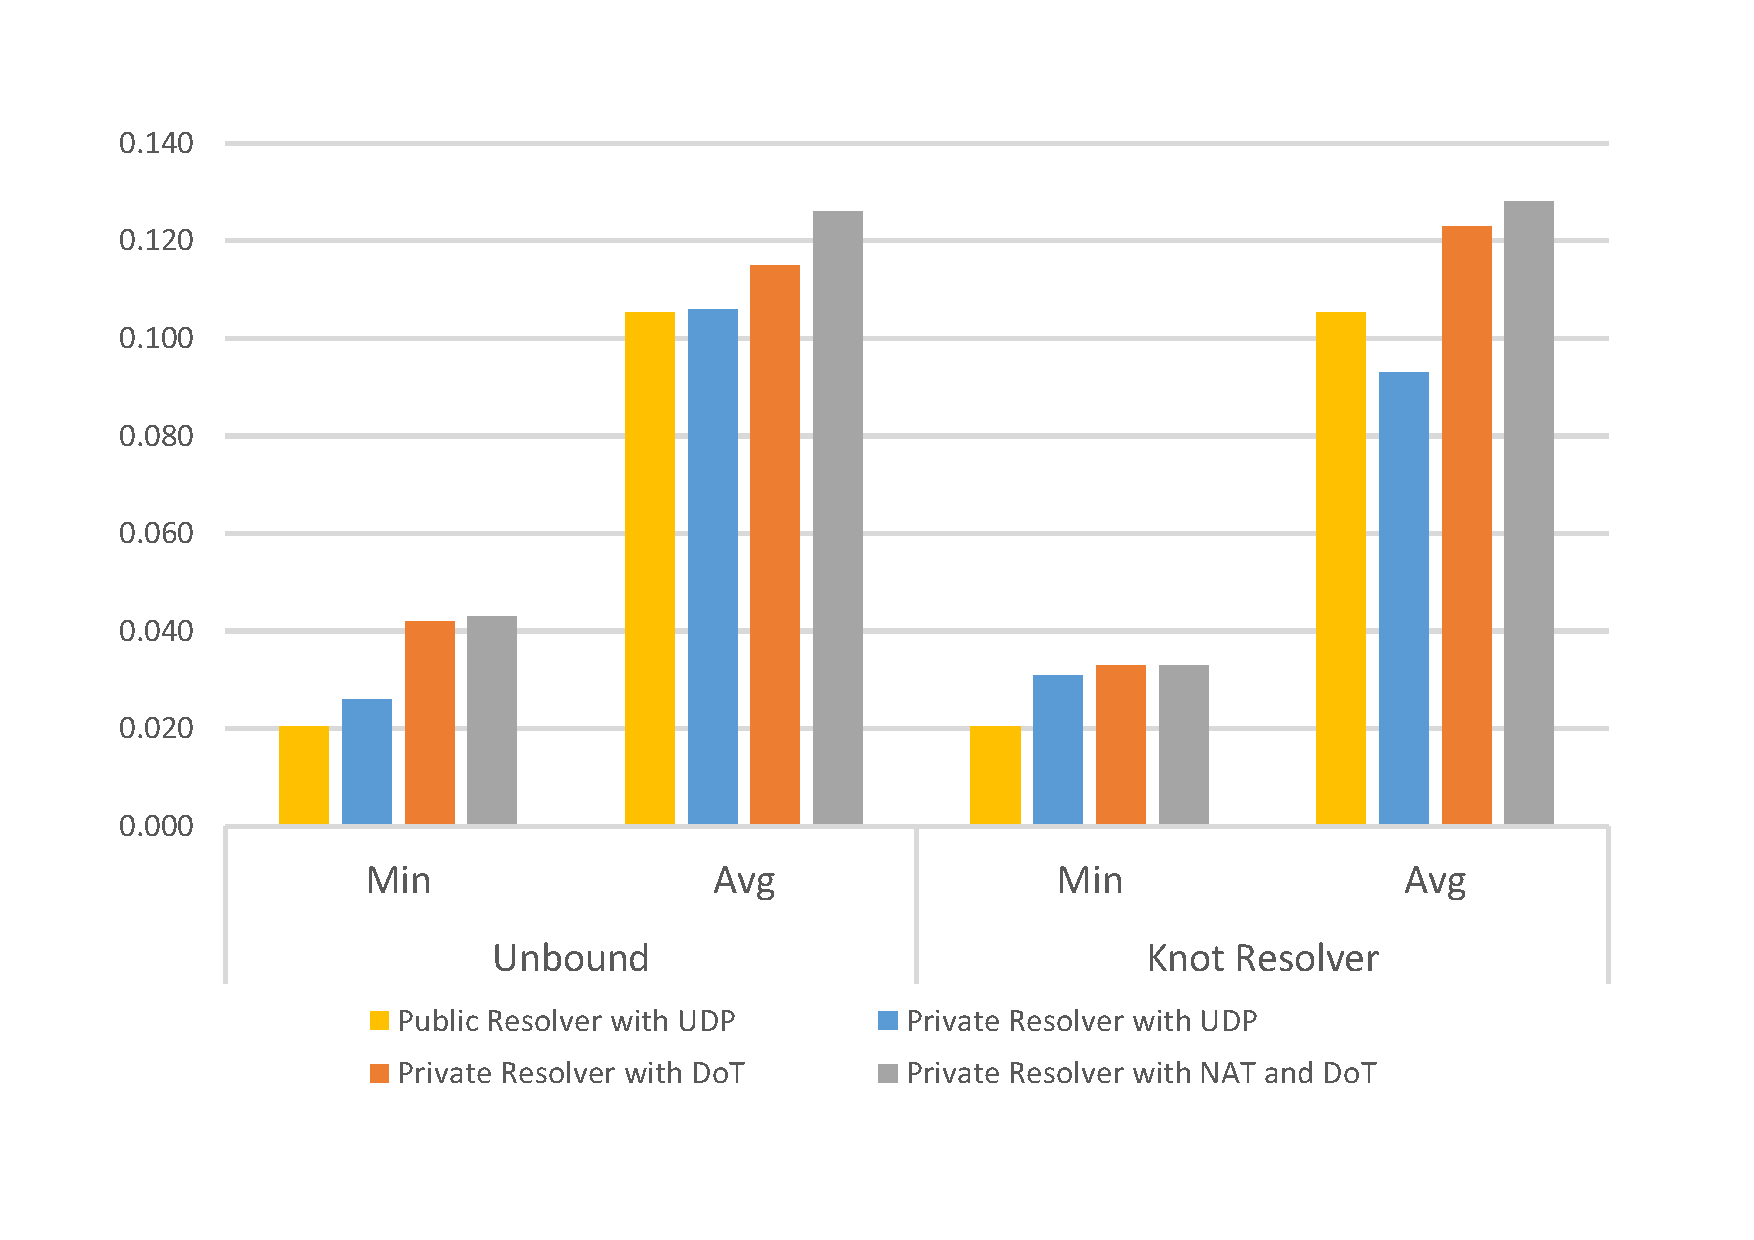
\includegraphics[width=0.6\textwidth]{Results_ResponseTimes}
    \caption{Balkendiagramm der Umlaufzeiten von DNS-Anfragen bei verschiedenen Varianten des dargelegten Aufbaus. Die Werte sind in Sekunden angegeben. Die Minimal- (min.) und Durchschnittswerte (avg.) ergeben sich aus Messungen mit dem Programm ``DNS Benchmark'' von Steve Gibson}
    \label{img:results-times}
\end{figure}

\chapter{Diskussion}
Betrachtet man das Konzept und den Test-Aufbau im Detail, können folgende Kritikpunkte ausgemacht werden. 

\paragraph{Sicheres lokales Netzwerk}
Der offensichtlichste Kritikpunkt ist die in Kapitel \ref{chap:implementation} angemerkte Annahme, dass kleine Netzwerke selten von innen heraus angegriffen werden. Diese Hypothese konnte im Zuge dieser Arbeit nicht verifiziert werden und bleibt daher Gegenstand möglichen zukünftiger Arbeiten. Geht man von einem unsicheren lokalen Netzwerk aus, ist die Kommunikation zwischen Client und lokalem DNS-Resolver weiterhin angreifbar. Dies ist auf die fehlende Unterstützung von sicheren Übertragungsprotokollen in aktuellen, in \acp{OS} integrierten Stub-Resolvern zurückzuführen. Der Einsatz von Local-Loopback Resolvern (wie in \ref{chap:implementation} beschrieben) wäre zwar eine mögliche Lösung, birgt jedoch verschiedene Probleme in der praktischen Realisierung.

\paragraph{Fingerprinting}
Ein anderer Punkt ist die Tatsache, dass die verwendeten Verfahren trotz starker Verschlüsselung anfällig auf Fingerprinting-Analysen zu sein scheinen \cite{Shulman2014}\cite{Siby2018}. Es werden zwei grundlegende Eigenschaften der Nachrichten untersucht: Größe und Timing. Es wird somit der Effekt ausgenutzt, dass der Zusammenhang zwischen frei beobachtbaren Eigenschaften signifikant genug ist, um einen Rückschluss auf bestimmte Anfragen zuzulassen. Dies könnte ausreichen, um die Privatsphäre der betroffenen Personen zu verletzen. Der inzwischen in Knot-Resolver implementierte Standard ``EDN0 Padding''\cite{rfc7830} ist dabei in der Lage, die wahre Größe verschlüsselter Nachrichten zu verschleiern. Außerdem wirkt sich der Einsatz von Trusted-Public-Resolvern positiv auf die Privacy aus, da sie die Analysen erschweren \cite{Shulman2014}. Ob diese Technik die vorgestellten Angriffe verhindert, werden jedoch erst zukünftige Arbeiten zeigen. 

\paragraph{DNS und HTTPS}
Darüber hinaus kann argumentiert werden, dass die Gefahren eines Angriffs auf DNS überschätzt werden. Diese Argumentationen stützt sich oft auf die immer weiter fortschreitende Verbreitung von HTTPS. Wird eine Webseite unter HTTPS veröffentlicht, würde eine DNS Spoofing Attacke aufgrund des fehlenden Zertifikats scheitern. Betrachtet man beispielsweise die in allen großen Browsern vertraute ``Let's Encrypt''-CA so stellt man fest, dass diese in ihrem Validierungsprozess eine sogenannte DNS-01-Challange anbietet. Durch diese ist es möglich, den Besitz einer Domäne über einen DNS-Eintrag zu beweisen. Es wäre einem Angreifer nun möglich aufgrund gezielter Angriffe auf den CA-DNS-Resolver ein valides Zertifikat zu erhalten. Dadurch stellt HTTPS keine Hürde bei einem Angriff dar und bietet eben keinen Schutz gegen DNS-Angriffe.

\chapter{Fazit}
\label{chap:conclusion}
Zusammenfassend kann gesagt werden, dass DNS als problematische Technologie von der IT-Security-Community erkannt wurde und seit vielen Jahren an verschiedensten Lösungsansetzen gearbeitet wird. Wie in Kapitel \ref{chap:threads} dargelegt wurde, sind die einzelnen Kernprobleme gut identifizierbar. Auch konkrete Bedrohungen durch Angriffe sind gut verstanden und über verschiedenste Methoden beleuchtet. Es konnte daher eine klare Aufzählung an Angriffskonzepten ausgearbeitet werden (siehe Kapitel \ref{chap:attacks}). Diese Darstellung der Gefahren für DNS-Clients wurde, zusammen mit bestehender Literatur, zur Erstellung eines Maßnahmenkatalogs (Kapitel \ref{chap:solutions}) verwendet. Dieser bot ein solides Grundgerüst zur Auswahl der in \ref{chap:technologies} näher beleuchteten Technologien. Abschließend konnte aufgrund dieser Auswahl ein praxistauglicher Aufbau getestet werden (Kapitel \ref{chap:implementation}). 

Die Ergebnisse der Performance- und Funktionstests bestätigten die Werte und Prognosen anderer Arbeiten und konnten zeigen, dass der Einsatz bestehender DNS-Sicherheits-Technologien durchaus möglich und tragbar ist. Durch das Aufkommen großer Trusted-Public-Resolver Projekte wie Google DNS, Cloudflare DNS und Quad9 wird eine performante und gleichzeitig sichere lokale DNS-Auflösung möglich und einfach zugänglich. 

Durch den Einsatz des in dieser Arbeit vorgestellten Konzepts lassen sich alle beschriebenen Sicherheitsprobleme von DNS vermeiden. Der Ressourcenaufwand wird dabei durch einen lokalen Resolver getragen. Da die Tests mit geringsten Hardware-Ressourcen (virtuell;1 vCPU; 1GB RAM) durchgeführt wurden, ist davon auszugehen, dass die Kosten für eine mögliche Umsetzung weit unter 100 Euro bleiben würden. Außerdem ist aufgrund des gewählten Modus von einem überaus geringen Wartungsaufwand auszugehen, was das Konzept zum sichern kleiner Netzwerke mit geringem Wartungsbudget prädestiniert.

Der gemessene Performanceverlust bei nicht gecachten Anfragen beläuft sich auf maximal 50-100\% Erhöhung der minimalen Umlaufzeiten, wobei sich die durchschnittliche Erhöhung auf lediglich 5-9\% beläuft  (siehe \ref{chap:results}). Je nach Anspruch kann sich dies zwar kritisch auf die Gesamtperformance der Clients auswirken, da sich diese Werte ausschließlich auf nicht gecachte Anfragen beziehen, ist davon auszugehen, dass sich diese Verzögerungen bei herkömmlicher Nutzung nicht negativ auf die User-Experience auswirken.

\paragraph{Ausblick}
Die aktuellen Entwicklungen lassen vermuten, dass sich der Funktionsumfang von Stub-Resolvern in Betriebssystemen \cite{Wallen2018} und Browsern \cite{McManus2018a} in Zukunft stark ändern könnte. Allgemein kann festgehalten werden, dass die in dieser Arbeit beschriebenen Probleme durch eine direkte Implementierung von sicheren Übertragungsprotokollen im Stub-Resolver einfacher und performanter lösbar werden. Da dies jedoch nur von den \ac{OS}- und Browserherstellern angestoßen werden kann, ist dies keine aktuell durchführbare Lösung. Die Zeit wird zeigen, ob das Thema DNS-Client-Security weitreichend genug ist, um die Aufmerksamkeit dieser Unternehmen und Gruppen zu gewinnen.  



% Literaturverzeichnis
\printbibliography
\clearpage

% Abbildungsverzeichnis
\listoffigures
\clearpage

% Tabellenverzeichnis
%\listoftables
%\clearpage

% Verzeichnis der Listings
\lstlistoflistings
\clearpage

% Abkürzungsverzeichnis
\phantomsection
\addcontentsline{toc}{chapter}{Abkürzungsverzeichnis}
\chapter*{Abkürzungsverzeichnis}
\begin{acronym}[XXXXXX]
    \acro{BSI}[BSI]{Bundesamt für Sicherheit in der Informationstechnik}
    \acro{CA}[CA]{Certificate Authority}
    \acro{CoT}[CoT]{Chain-Of-Trust}
    \acro{DJB}[DJB]{Daniel J. Bernstein}
    \acro{DNSSEC}[DNSSEC]{Domain Name System Security Extensions}
    \acro{DNS}[DNS]{Domain Name System}
    \acro{DoH}[DoH]{DNS-over-HTTPS}
    \acro{DoS}[DoS]{Denial-Of-Service}
    \acro{DoT}[DoT]{DNS-over-TLS}
    \acro{ECC}[ECC]{Elliptic Curve Cryptography}
    \acro{HTTPS}[HTTPS]{Hypertext Transfer Protocol Secure}
    \acro{HTTP}[HTTP]{Hypertext Transfer Protocol}
    \acro{IANA}[IANA]{Internet Assigned Numbers Authority}
    \acro{IETF}[IETF]{Internet Engineering Task Force}
    \acro{ISP}[ISP]{Internet Service Providers}
    \acro{MAC}[MAC]{Message Authentication Code}
    \acro{MITM}[MITM]{Man-In-The-Middle}
    \acro{MTU}[MTU]{Maximum Transmission Unit}
    \acro{NAT}[NAT]{Network Address Translator}
    \acro{NTP}[NTP]{Network Time Protocol}
    \acro{ODNS}[ODNS]{Oblivious DNS}
    \acro{OS}[OS]{Betriebssystem}
    \acroplural{OS}[OS]{Betriebssystemen}
    \acro{PKI}[PKI]{Public Key Infrastructure}
    \acro{RRset}[RRset]{Ressource Record Set}
    \acro{RR}[RR]{Ressource Record}
    \acro{SLD}[SLD]{Second Level Domain}
    \acroplural{SLD}[SLDs]{Second Level Domains}
    \acro{SSH}[SSH]{Secure Shell}
    \acro{T-DNS}[T-DNS]{DNS-over-TCP}
    \acro{TLD}[TLD]{Top Level Domain}
    \acroplural{TLD}[TLDs]{Top Level Domains}
    \acro{TLS}[TLS]{Transport-Layer-Security}
    \acro{TOFU}[TOFU]{Trust-On-First-Use}
    \acro{TTL}[TTL]{Time-To-Live}
    \acro{TXID}[TXID]{Transaktions-ID}
    \acro{WWW}[WWW]{World Wide Web}
\end{acronym}

%Anhänge
\lstset{ 
  basicstyle=\tiny\ttfamily,
  linewidth=14cm,
  xleftmargin=2cm
}

\chapter*{Anhang A}
\label{chap:appA}
In diesem Anhang werden die für die Reproduktion notwendigen Konfigurationsdateien zur Verfügung gestellt. 

Das Nachfolgende Listing stellt das Konfigurationsscript für die Host-Firewall des Servers dar. Es wurde dabei ein minimales Setup gewählt. Dabei sind nur die notwendigen ein- und ausgehenden Verbindungen berechtigt.

\lstinputlisting[language=Bash]{code/set-fw.sh}
\clearpage

Die Konfigurationsdatei \texttt{/etc/unbound/unbound.conf} des Unbound 1.4.7 Servers ist in folgendem Listing festgehalten. Die Kommentare ab Zeile 41 stellen die einzelnen Betriebsmodi dar. Zum aktivieren einfach die aktuellen Zeilen aus- und die anderen einkommentieren. Achtung! Der Teil \texttt{\#dns.quad9.net} hinter den Zeilen beginnend mit \texttt{forward-addr:} sind keine Kommentare sondern die Hostnamen für die Validierung der TLS-Zertifikate. 

\lstinputlisting[language=Bash]{code/unbound.conf}
\clearpage

Diese Listing folgt dem von oben, betrifft hier nur die Knot-Resolver-Config unter \texttt{/etc/knot-resolver/}.

\lstinputlisting[language={[5.0]Lua}]{code/kresd.conf}

%spellcheck-off
\chapter*{Anhang B}
\label{chap:appB}

Die nachfolgende Tabelle zeigt die Rohdaten der Messergebnisse der Software ``DNS Benchmark''. Die Zahlenwerte zeigen die minimale (min), durchschnittliche (avg) und maximale (max) RTT, sowie deren Standardabweichung (Std.Dev) sowie die Erfolgsrate von 10 ausgewählten Open-Recursive-Resolvern. Diese Werte wurden als Durchschnitte zur Errechnung eines Vergleichswerts für die in Kapitel \ref{chap:results} vorgestellten Ergebnisse verwendet.

\begin{table}[ht]
\centering
\begin{tabular}{lllllll}
\hline
Resolver IP    & Min   & Avg   & Max   & Std.Dev & Reliab[\%] \\ \hline
129.250.35.250 & 0.009 & 0.012 & 0.022 & 0.002   & 100.0    \\
129.250.35.251 & 0.009 & 0.012 & 0.017 & 0.001   & 100.0    \\
1.1.1.1        & 0.009 & 0.013 & 0.017 & 0.002   & 100.0    \\
9.9.9.9        & 0.010 & 0.013 & 0.023 & 0.002   & 100.0    \\
1.0.0.1        & 0.014 & 0.017 & 0.023 & 0.002   & 100.0    \\
8.8.8.8        & 0.016 & 0.019 & 0.024 & 0.002   & 100.0    \\
8.8.4.4        & 0.015 & 0.019 & 0.027 & 0.002   & 100.0    \\
4.2.2.4        & 0.021 & 0.024 & 0.029 & 0.002   & 100.0    \\
4.2.2.6        & 0.021 & 0.024 & 0.030 & 0.002   & 100.0    \\
4.2.2.1        & 0.021 & 0.026 & 0.032 & 0.003   & 100.0    \\ \hline
\end{tabular}
\caption*{Daten aus der Vergleichswertemessung. Werte in Sekunden.}
\end{table}

\end{document}